\providecommand{\toplevelprefix}{../..}  % necessary for subfile bibliography + figures compilation to work, do not move this after documentclass

\documentclass[../../book-main_zh.tex]{subfiles}

\graphicspath{{\subfix{../..}}}
\begin{document}

\chapter{一致性与自洽性表示}
\label{ch:consistent}\label{ch:autoencoding}
\label{ch:self-consistent}\label{ch:closed-loop}

\begin{quote}
\hfill  “{\em 任何事情都应该做得尽可能简单,但不能再简单了}。”

$~$\hfill -- 阿尔伯特·爱因斯坦
\end{quote}

% \begin{quote}
%   \hfill  “{\em 自20世纪80年代以来,显而易见的是,
%     通过深度自编码器进行反向传播对于非线性降维将非常有效,
%     前提是计算机足够快,数据集足够大,并且初始
%     权重足够接近一个好的解决方案。所有这三个条件
%   现在都已满足}。”

%   $~$\hfill -- Geoffrey Hinton and Ruslan  Salakhutdinov, 2006
% \end{quote}

\vspace{5mm}


在前面的章节中,我们建立了一个基本事实,即学习的
根本目标是学习一个具有低维支撑的数据
分布,并将其转换为一个紧凑且结构化的
表示。这样的表示揭示了数据分布的内在
低维结构,并为后续任务(如分类和生成)提供了便利。

学习这种分布的良好表示的一个基本方法是通过{\em 压缩}。为了使压缩的
目标可度量和可计算,可以通过
学习一个编码方案来明确地实现,该方案最小化编码率(熵)或最大化信息增益(编码率
缩减)。在这种背景下,深度神经
网络的基本作用是实现某种迭代优化算法,
该算法根据这些度量逐步优化学习到的表示:
\begin{equation}
  f\colon \X
  \xrightarrow{\hspace{1mm} f^0 \hspace{1mm}} \Z^0 \rightarrow \cdots
  \rightarrow \Z^\ell \xrightarrow{\hspace{1mm} f^\ell \hspace{1mm}}
  \Z^{\ell+1} \rightarrow  \cdots \to \Z^L = \Z.
\end{equation}
在上一章中,我们已经表明,几乎所有流行的深度网络(ResNet、CNN 和
Transformer)的主要架构
特征都可以从这个角度推导和解释。

然而,当我们试图通过
优化达到某个目标时,并不能保证
通过增量优化最终找到的解 $\Z$ 是正确的解。事实上,即使
优化过程设法找到了全局最优
解 $\Z^*$,也不能保证该解对应
于数据分布的完整表示。\footnote{这可能由多种原因引起:例如,用于学习分布的数据可能不足,或者优化问题的公式未能考虑一些额外的约束或条件。}因此,一个悬而未决的问题是我们如何能确保学习到的数据分布的表示是
正确或足够好的?

当然,验证这一点的唯一方法是看是否存在一个解码映射,比如说 $g$,能够将学习到的表示解码以足够好地再现原始数据(分布):
\begin{equation}
  \X
  \xrightarrow{\hspace{1mm} \mathcal{E} = f \hspace{1mm}} \Z
  \xrightarrow{\hspace{1mm} \mathcal{D} = g \hspace{1mm}} \hat{\X}
\end{equation}
这需要通过某种相似性度量:
\begin{equation}
  d(\X, \hat \X).
\end{equation}
这引出了{\em 一致性表示}的概念。正如我们在
\Cref{ch:intro} 中简要提到的(见 \Cref{fig:autoencoder}),{\em 自编码}整合了
编码和解码过程,是学习这种表示的自然框架。我们已经在 \Cref{ch:classic} 中研究了一些重要的特例。在
本章的 \Cref{sec:consistent-representation} 中,我们将研究如何通过强制 $\X$ 和 $\hat \X$ 之间的一致性,将自编码扩展到更一般的分布类别。

在许多实际和自然的学习场景中,比较数据 $\X$ 和 $\hat \X$ 的分布可能很困难甚至不可能。我们只剩下唯一的选择,即在学习到的特征 $\Z$ 中,将其与它在编码器 $f$ 下的像 $\hat \Z$ 进行比较:
\begin{equation}
 \X
\xrightarrow{\hspace{1mm} \mathcal{E} = f \hspace{1mm}} \Z  \xrightarrow{\hspace{1mm} \mathcal{D} = g \hspace{1mm}} \hat{\X} \xrightarrow{\hspace{1mm} \mathcal{E} = f \hspace{1mm}} \hat \Z?
\end{equation}
这引出了{\em 自洽性表示}的概念。在 \Cref{sec:self-consistency} 中,我们将研究何时以及如何仅通过闭环转录框架,强制 $\Z$ 和 $\hat \Z$ 之间的自洽性来学习一致性表示。

此外,在许多实际和自然的学习场景中,我们通常不会一次性拥有数据分布的足够样本。例如,动物和人类通过一生中不断地接收增量的观察来发展他们的视觉记忆。在 \Cref{sec:continuous} 中,我们将研究如何扩展闭环转录框架,以在{\em 持续学习}设置中学习自洽性表示。

当然,我们想要识别
数据分布中的低维结构并找到一个良好
表示的一个根本动机是,为了更容易地将数据用于各种智能
任务,例如分类、补全和预测。
因此,得到的联合表示 $(\x, \z)$ 必须以最适合这些任务的方式进行结构化。在
下一章中,我们将
看到如何结构化学习到的表示,以促进
条件补全或生成任务。

\section{学习一致性表示}\label{sec:consistent-representation}
%\yima{重写此部分以清晰地陈述数学问题,
% 包括假设(例如充分性)和目标。讨论
% 可计算和可实现的目标的近似或变体。}

这里我们给出一致性表示的正式定义,它
与自编码的概念密切相关。%\yima{也许我们
% 想为两种一致性类型分开定义:
% 样本级与分布级。}
\begin{definition}[一致性表示]\label{def:bidirectional_rep}
  给定数据 \(\vX\),一个\textit{一致性表示}是一对
  函数 \((f \colon \cX \to \cZ, g \colon \cZ \to \cX)\),使得
  \textit{特征} \(\vZ = f(\vX)\) 是紧凑且
  结构化的,并且\textit{自编码}
  \begin{equation}
    \hat{\vX} \doteq g(\vZ) = g(f(\vX))
  \end{equation}
  根据以下两种度量之一,与 \(\vX\) \textit{接近}:
  \begin{enumerate}
    \item 如果 \(\vX
      \approx \hat{\vX}\) 在某种范数下以高概率成立,我们说它是\textit{样本级}一致的。
    \item 如果 \(\Law(\vX) \approx \Law(\hat{\vX})\),我们说该表示是\textit{分布级
      一致的}。
  \end{enumerate}
\end{definition}
%\sdb{与感知与失真相关。}

敏锐的读者可能已经注意到,如果我们不对所寻求的表示 $\Z$ 施加某些
要求,上述问题将有一个
平凡解:我们可以简单地选择函数 $f$ 和 $g$
为恒等映射!因此,寻求
自编码的真正目的是试图确保如此获得的 $\Z$ 比 $\X$ 更
紧凑、更结构化。首先,为了紧凑性,$\Z$
应该更好地揭示 $\X$ 的内在低维性。
因此,表示应该最大化某种信息
增益,例如,用在 \Cref{subsec:MCR2} 中引入的率差
\begin{equation}
  \Delta R_{\epsilon}(\Z)
\end{equation}
来衡量。其次,
学习数据分布的良好表示的主要目的是
促进利用其分布的低维性的任务。
因此,$\Z$ 的分布应该更好地结构化。例如,$\Z$ 的分布是分段线性的
或高斯的,其分量在很大程度上是不相干或独立的
等等。这些独立的分量可以代表不同的簇或
类别,也可以很容易地用作解码
相应数据 $\x$ 的条件。

从一致性表示的定义来看,它要求
表示 $\Z$ 足以在一定程度上恢复原始数据
分布 $\X$。对于样本级
一致性,一个典型的选择是最小化期望重构误差:
\begin{equation}
  d(\X, \hat \X) = \mathbb{E}[\|\X - \hat\X\|_2^2].
\end{equation}
对于分布上的一致性,一个典型的选择是最小化
某个分布距离,例如KL
散度\footnote{请注意,对于没有共同
  支撑的分布,这对于退化分布是典型的,KL散度
  甚至可能没有很好的定义。事实上,许多分布
  学习文献正试图通过
  用定义良好且可有效计算的东西来替换或近似它来解决这个技术难题。}:
\begin{equation}
  d(\X, \hat \X) = \mathcal{D}_{KL}(\X\|\hat\X).
\end{equation}

因此,撇开计算不谈,当我们为数据
分布 $\X$ 寻求一个好的自编码时,概念上我们试图找到一个编码器 $f$ 和
解码器 $g$,使得
\begin{equation}
  \min_{f, g} [- \Delta R_{\epsilon}(\Z) + d(\X, \hat \X)].
  \label{eqn:autoencode-objective-ch5}
\end{equation}
%\sdb{最大化 $\Delta R$?}
在本章的其余部分,我们将研究如何在不同条件下解决此类
自编码问题,从简单和
理想的情况到越来越具有挑战性和现实性的条件。

%\section{从线性到非线性自编码}\label{sec:NLPCA}
%\yima{如何确保表示是紧凑和结构化的,
% 比如说线性或分段线性,或信息丰富的?经典的
% 自编码器没有明确施加这样的... 增量
% 展平变换,特别是
% \href{https://arxiv.org/abs/2305.01777}{非线性流形
% 展平和重构}。这是一个样本级重构
% 一致性的例子。}

\subsection{通过PCA实现的线性自编码}
根据 \cite{Baldi2011},短语“自编码器”最早
由 Hinton 和 Rumelhart \cite{Rumelhart1986} 提出,以便通过反向传播(BP)以自监督的方式学习
深度表示——重构原始数据是自监督任务。然而,寻求紧凑和一致表示的
这一概念早已植根于许多经典研究中。正如我们在 \Cref{ch:classic} 中已经看到的,经典的主成分分析(PCA)、独立成分分析(ICA)和稀疏字典学习都有类似的目标。唯一的区别是,当底层数据分布简单(线性和
独立)时,编码或解码映射变得易于表示和
学习:它们不需要是深度的,并且通常可以以封闭形式或
通过显式算法计算。

在我们定义的简单PCA案例中,看看一致性的概念是如何发挥作用的,是很有启发性的:
这里,一致的编码和解码映射由单层
线性变换给出:
\begin{equation}
  \X \xrightarrow{\hspace{2mm} \mathcal{E} = \vU^\top \hspace{2mm}}
  \Z \xrightarrow{\hspace{2mm} \mathcal{D} = \vU \hspace{2mm}}   \hat{\X},
  \label{eqn:autoencoding-PCA-2}
\end{equation}
其中 $\vU \in \mathbb{R}^{D\times d}$ 通常 $d\ll D$。因此
$\vU^\top$ 表示从高维空间
$\mathbb{R}^{D}$ 到低维空间 $\mathbb{R}^{d}$ 的投影,如
\Cref{fig:AE} 所示。
\begin{figure}
  \centering \includegraphics[width=0.5\linewidth]{\toplevelprefix/chapters/chapter5/figs/autoencoder.png}
  \caption{一个典型自编码器(如PCA)的图示,它为高维数据 $\vx$ 寻找
  一个低维表示 $\bm{z}$。}
  \label{fig:AE}
\end{figure}

正如我们在 \Cref{ch:classic} 中看到的,当 $\vx$ 的分布确实
支撑在一个低维子空间 $\vU_o$ 上时,由 $\cE$ 产生的表示
$\vz$ 的紧凑性是正确
估计(并强制)该子空间维度的直接结果。最后,
回想一下,在重构准则上的梯度下降恰好
产生这些样本级一致的映射:实际上,问题
\begin{equation}\label{eq:pca-reconstruction-ch5}
  \min_{\vU^\top \vU = \vI}\, \bE_{\vx}\left[\norm*{\vx
  - \vU\vU^\top \vx}_2^2\right]
\end{equation}
的最优解在表示的维度
足够大时,恰好与 $\vU_o$ 一致。在这种情况下,我们免费获得了样本级一致性,
因为这保证了 $\vU_o\vU_o^\top \vx = \vx$。
请注意,在PCA的情况下,
\eqref{eqn:autoencode-objective-ch5} 中的率差项变得无效,因为对所寻求的表示 $\Z$ 的正则化是显式的:它跨越了整个
低维子空间\footnote{在这种情况下,可以认为 $\Delta R = 0$。}。

\paragraph{在线PCA。} 请注意,在上述构造中,用于编码和解码的
线性变换 $\vU$ 是事先从所有
输入数据中“离线”计算的。一个问题是,这个变换
是否可以随着输入数据的顺序到来而“在线”学习?这个问题
在1982年由Oja的工作 \cite{Oja1982SimplifiedNM} 回答了。
\begin{example}[PCA的归一化赫布学习方案] 考虑
  一系列i.i.d.随机向量 $\x_1, \ldots, \x_i, \ldots \in
  \mathbb{R}^n$,其协方差为 $\boldsymbol{\Sigma} \in
  \mathbb{R}^{n\times n}$。令 $\vu_0 \in \mathbb{R}^n$ 并定义
  输入向量 $\x_i$ 对权重向量
  $\vu_i$ 的响应为其内积:
  \begin{equation}
    \eta_i = \vu_i^T \x_i
  \end{equation}
  我们根据以下方案更新权重向量:
  \begin{equation}
    \vu_{i+1} = \frac{\vu_i + \gamma \eta_i \x_i}{\|\vu_i + \gamma
    \eta_i \x_i\|_2}
    \label{eqn:Hebbian}
  \end{equation}
  对于某个小的增益 $\gamma >0$。这个更新方案可以看作
  是一个归一化的赫布方案,其中神经元之间的连接
  权重如果输入 $\x$ 和输出 $\eta$ 的(乘积)都很强,则会变得更强。可以认为权重向量
  $\vu$ 是基于
  输出 $\eta$ 的某种形式的反馈而“学习”的。
  然后,在合理的假设下,Oja \cite{Oja1982SimplifiedNM} 已经
  证明了 $\vu_i$ 收敛到与 $\boldsymbol{\Sigma}$ 的
  大特征值相关联的特征向量。
\end{example}

归一化的赫布方案 \eqref{eqn:Hebbian} 可以被解释为
在问题 \eqref{eq:pca-reconstruction-ch5} 的目标上(批量大小为
$1$,且 $\vU$ 的列数为 $1$)进行\textit{随机}投影
梯度下降方案的一阶近似,只要
$\norm{\vu}_2 = 1$,这一点由
\eqref{eqn:Hebbian} 中的投影操作来维持。
记住它的存在是值得的,既作为
使用随机梯度方法优化
重构成本(如 \eqref{eq:pca-reconstruction-ch5})的正确性证明,也因为它
暗示了\textit{比(端到端)反向
  传播更简单的算法可以
成功学习一致性自编码器}。

\begin{figure}
  \centering
  % \includegraphics[width=12cm]{interpolate.jpg}
  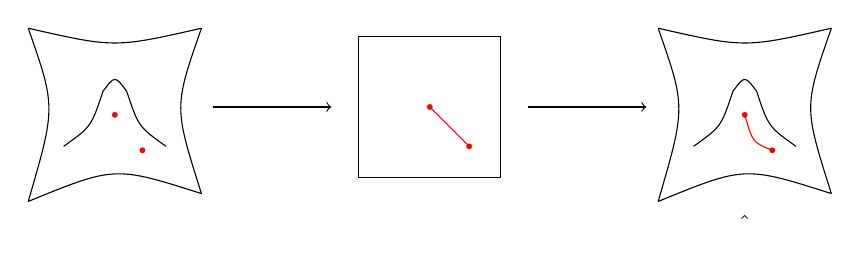
\begin{tikzpicture}
    \draw (-0.1, -0.2) .. controls (1, 0.25) .. (2.1, -0.1);
    \draw (2.1, -0.1) .. controls (1.75, 1) .. (2.1, 2);
    \draw (2.1, 2) .. controls (1, 1.75) .. (-0.1, 2);
    \draw (-0.1, 2) .. controls (0.25, 1) .. (-0.1, -0.2);

    \draw (0.35, 0.5) .. controls (0.7, 0.75) .. (0.85, 1.2);
    \draw (0.85, 1.2) .. controls (1.0, 1.4) .. (1.15, 1.2);
    \draw (1.15, 1.2) .. controls (1.3, 0.75) .. (1.65, 0.5);

    \node[fill, red, circle, inner sep=0.75pt] at (1, 0.9) {};
    \node[fill, red, circle, inner sep=0.75pt] at (1.35, 0.45) {};

    \node at (1, -0.5) {\(\x\)};

    \draw[->] (2.25, 1) -- (3.75, 1);
    \node at (3, 1.25) {\(\fl\)};

    \draw (4.1, 0.1) -- (5.9, 0.1);
    \draw (5.9, 0.1) -- (5.9, 1.9);
    \draw (5.9, 1.9) -- (4.1, 1.9);
    \draw (4.1, 1.9) -- (4.1, 0.1);

    \node[fill, red, circle, inner sep=0.75pt] at (5, 1) {};
    \node[fill, red, circle, inner sep=0.75pt] at (5.5, 0.5) {};

    \draw[red] (5, 1) -- (5.5, 0.5);

    \node at (5, -0.5) {\(\z\)};

    \draw[->] (6.25, 1) -- (7.75, 1);
    \node at (7, 1.25) {\(\re\)};

    \draw (7.9, -0.2) .. controls (9, 0.25) .. (10.1, -0.1);
    \draw (10.1, -0.1) .. controls (9.75, 1) .. (10.1, 2);
    \draw (10.1, 2) .. controls (9, 1.75) .. (7.9, 2);
    \draw (7.9, 2) .. controls (8.25, 1) .. (7.9, -0.2);

    \draw (8.35, 0.5) .. controls (8.7, 0.75) .. (8.85, 1.2);
    \draw (8.85, 1.2) .. controls (9.0, 1.4) .. (9.15, 1.2);
    \draw (9.15, 1.2) .. controls (9.3, 0.75) .. (9.65, 0.5);

    \node[fill, red, circle, inner sep=0.75pt] at (9, 0.9) {};
    \node[fill, red, circle, inner sep=0.75pt] at (9.35, 0.45) {};

    \draw[red] (9, 0.9) .. controls (9.1, 0.55) .. (9.35, 0.45);

    \node at (9, -0.5) {\(\hat{\x}\)};
  \end{tikzpicture}
  \caption{在\(\R^{3}\)中一个维度为\(d = 2\)的流形上通过流形展平进行插值的描绘。要在数据流形上插值
    两个点,通过展平映射\(\fl\)将它们映射到展平空间,取它们的凸插值,
    然后通过重构映射\(\re\)将它们映射回数据流形。}
  \label{fig:idealized_interpolation}
\end{figure}

\subsection{非线性PCA和自编码}\label{sub:nonlinear-pca}\label{sec:NLPCA}
当然,当我们处理更复杂的分布时,其潜在的
低维结构可能是非线性的,我们应该预料到事情将不再那么简单。

\paragraph{非线性子流形上的数据。} 因此,为了超越
PCA处理的线性结构,我们可以假设数据分布位于一个(光滑的)子流形 $\mathcal{M}$ 上。子流形的内在维度,比如说 $d$,通常远低于
环境空间 $\mathbb{R}^D$ 的维度。从这个几何
角度来看,我们通常希望找到一个非线性映射 $f$,使得
得到的流形
$f(\mathcal{M})$ 被展平,如 \Cref{fig:idealized_interpolation} 所示的例子。得到的特征 $\vz$-空间
通常
比 $\vx$-空间更紧凑(维度更低),并且
流形是平坦的。
从统计学的角度,这与几何
角度互补但在一般情况下是不同的,我们可能还希望确保 $\cM$ 上的数据
分布被映射到一个足够规则的
分布,比如说高斯分布或均匀分布(具有一个
非常低维的支撑),在 $\vz$-空间中。这两个属性确保了在 $\vz$-空间中的采样和插值尽可能容易,它们是对数据分布的低维流形
模型中理想的
紧凑和结构化特征概念的数学形式化。
总的来说,为这类
数据分布学习这样一个自编码映射的问题被称为{\em 非线性主成分分析}
(NLPCA)。

\paragraph{通过两层网络的经典尝试。} 正如我们
上面看到的,在PCA的情况下,一个单层的线性神经
网络就足够了。对于NLPCA来说,情况不再如此。1991年,Kramer
\cite{Kramer1991NonlinearPC} 提出使用一个两层
神经网络来表示编码器映射 $f$(或其逆 $g$),基于带有sigmoid
激活函数的两层网络的通用表示属性:
\begin{equation}
  \z = \vW_2 \sigma(\vW_1\x +\vb),
\end{equation}
其中 $\sigma(\spcdot)$ 是sigmoid函数:
\begin{equation}
  \sigma(x) = \frac{1}{1+ e^{-x}}.
\end{equation}
Cybenko \cite{Cybenko1989ApproximationBS} 表明,
上述形式的函数(具有足够的隐藏节点)可以以任意
精度逼近任何光滑的
非线性函数,比如说编码器 $f(\spcdot)$。特别是,它们可以表示
支撑在(低维流形的并集上的)数据分布的展平和重构
映射,
如 \Cref{fig:idealized_interpolation} 所示。
Kramer提出的
原始网络的整体架构如图 \Cref{fig:NLPCA} 所示。
\begin{figure}[tb]
  \centering
  \includegraphics[width=0.6\linewidth]{\toplevelprefix/chapters/chapter5/figs/kramer1991nonlinearPCA.png}
  \caption{Kramer \cite{Kramer1991NonlinearPC} 建议的,通过用于编码和解码映射的深度
    为二的自联想神经网络进行的非线性PCA。}
  \label{fig:NLPCA}
\end{figure}

不幸的是,与上述PCA的情况不同,这些网络的参数 $\boldsymbol{\theta} =
(\vW, \vb)$ 通常没有
封闭形式的学习方案。因此,有人提出通过反向传播来训练
网络,并以重构误差作为监督:
\begin{equation}\label{eq:nonlinear-pca-ch5}
  \min_{\boldsymbol{\theta}} \mathbb{E}[ \|\x - \hat{\x}(\boldsymbol{\theta})\|_2^2].
\end{equation}
与PCA的简单情况相比,我们利用相同的重构目标
进行学习,但使用一个远为复杂的非线性模型类来
参数化和学习编码器和解码器。尽管通用
近似属性(如Cybenko的)表明,\textit{原则上}
通过这个框架学习一致性自编码器是可能的——因为对于
任何随机数据样本,给定足够的参数,这样的自编码对
是存在的——但人们通常发现用梯度下降找到它们是非常不平凡的。
此外,为了获得一个足够信息丰富的重构目标
和高维真实世界数据(如图像)的分布
模型,所需的
样本和隐藏节点的数量可能非常巨大。
此外,作为学习表示紧凑性的度量,瓶颈层的
$\z$ 的(较低)维度通常是
启发式选择的。\footnote{在后来的工作 \cite{Hinton-1993} 中,Hinton等人
  建议使用最小描述长度(MDL)原则来促进
  学习的编码方案的紧凑性,其精神与本书中介绍的
率失真度量非常相似。}
% \sdb{我们也可以在这里连接到Oja的理论:我们用BP学习(不只是调用GD)
% + 它变得非局部...}

\paragraph{通过更深层次的网络进行流形展平。}
基于深度网络的现代实践,这种经典的浅层
宽网络架构被认为通过反向传播(BP)进行有效和高效的训练是相当困难的,部分
原因是sigmoid函数的梯度消失问题。因此,
现代实践通常建议进一步
将非线性变换 $f$(或 $g$)分解为
更多层更简单变换的组合,从而产生更深的网络架构
\cite{Hinton504},如 \Cref{fig:ccnet_layers} 所示。
在现代背景下,对基本重构成本
\eqref{eq:nonlinear-pca-ch5} 的进一步阐述也被证明是必要的,以便在
复杂的真实世界数据分布(如图像)上取得良好性能。

\begin{figure}[htb]
  \centering
  \begin{tikzpicture}
    \draw (-0.1, -0.2) .. controls (1, 0.25) .. (2.1, -0.1);
    \draw (2.1, -0.1) .. controls (1.75, 1) .. (2.1, 2);
    \draw (2.1, 2) .. controls (1, 1.75) .. (-0.1, 2);
    \draw (-0.1, 2) .. controls (0.25, 1) .. (-0.1, -0.2);

    \draw (0.35, 0.5) .. controls (0.7, 0.75) .. (0.85, 1.2);
    \draw (0.85, 1.2) .. controls (1.0, 1.4) .. (1.15, 1.2);
    \draw (1.15, 1.2) .. controls (1.3, 0.75) .. (1.65, 0.5);

    \node at (1, -0.5) {\(\x\)};

    \draw[->] (2.25, 1.25) -- (3.25, 1.25);
    \node at (2.75, 1.5) {\(\fl_{1}\)};

    \draw[->] (3.5, 1.25) -- (4.5, 1.25);
    \node at (4, 1.5) {\(\fl_{2}\)};

    \draw[->] (4.75, 1.25) -- (5.75, 1.25);
    \node at (5.25, 1.5) {\(\cdots\)};

    \draw[->] (6, 1.25) -- (7, 1.25);
    \node at (6.5, 1.5) {\(\fl_{L}\)};

    \draw[->] (7, 0.75) -- (6, 0.75);
    \node at (6.5, 0.5) {\(\re_{L}\)};

    \draw[->] (5.75, 0.75) -- (4.75, 0.75);
    \node at (5.25, 0.5) {\(\cdots\)};

    \draw[->] (4.5, 0.75) -- (3.5, 0.75);
    \node at (4, 0.5) {\(\re_{2}\)};

    \draw[->] (3.25, 0.75) -- (2.25, 0.75);
    \node at (2.75, 0.5) {\(\re_{1}\)};

    \draw (7.3, 0.1) -- (9.1, 0.1);
    \draw (9.1, 0.1) -- (9.1, 1.9);
    \draw (9.1, 1.9) -- (7.3, 1.9);
    \draw (7.3, 1.9) -- (7.3, 0.1);

    \node at (8.2, -0.5) {\(\z\)};

  \end{tikzpicture}
  \caption{展平
    和重构对 \((\fl, \re)\) 的构造过程的描绘,其中编码器 \(\fl =
    \fl_{L} \circ \fl_{L - 1} \circ \cdots \circ \fl_{1}\) 是
    由组合展平层构成的,而解码器 \(\re
    = \re_{1} \circ \re_{2} \circ \cdots \circ \re_{L}\) 是由
  每个 \(\fl_{\ell}\) 的逆组成的。}
  \label{fig:ccnet_layers}
\end{figure}

鉴于像Cybenko这样的通用近似定理,人们
最初可能会想知道,为什么从概念上讲,更深的自编码器应该优于
浅层的自编码器。
从纯粹的表达能力角度,我们可以通过
与展平我们假设数据分布所在的非线性
流形任务相关的几何角度来理解这种现象。一种纯粹
构造性的流形展平方法是增量进行的,
与我们在 \Cref{ch:compression,ch:representation} 中看到的
扩散、去噪和压缩之间的相互作用并行。在几何
设置中,对应于 $f_{\ell}$ 的增量\textit{展平过程}
的形式是将流形上一点的邻域变换为
更接近平坦流形(即子空间)的形式,并强制与
其余数据样本的局部一致性;解码器中相应的增量操作
$g_{\ell}$ 则撤销此变换。此过程精确地
包含了关于底层流形的曲率信息,该信息是
从数据样本中估计的。给定足够的流形样本和
对这个概念过程的仔细实例化,有可能将
此过程实现为一个可验证地以白盒方式展平非线性
流形的计算过程 \cite{Psenka-JMLR24}。然而,该方法
由于可扩展性不佳,在应用于高维数据分布(如
图像)时受到限制,这促使了更
灵活的增量自编码方法的发展。

\subsection{稀疏自编码}
在上述自编码方案中,特征空间的维度
$d$ 通常被选择为远低于原始数据
空间 $D$ 的维度,以便明确地强制或促进学习到的
表示是低维的。然而,在实践中,我们
通常不知道数据的内在维度
分布。因此,为
自编码选择特征空间维度通常是凭经验完成的。在更一般的情况下,
数据分布可以是少数低维
子空间或子流形的混合。在这些情况下,不再可行
为所有特征强制一个单一的低维空间。

稀疏自编码器旨在解决这些限制中的一些。特别地,特征空间的维度可以等于甚至
高于数据空间的维度,如
\Cref{fig:SAE} 所示。然而,特征被要求在特征空间中高度
稀疏。因此,如果我们在目标
\eqref{eqn:autoencode-objective-ch5} 中除了率差之外,还施加稀疏性作为
简约性的度量,我们得到一个稀疏自编码的新目标:
\begin{equation}
  \min_{f, g}
  %\lambda
  [\|\Z\|_0 - \Delta R_{\epsilon}(\Z) + d(\X, \hat \X)],
  \label{eqn:autoencode-sparse}
\end{equation}
其中 $\ell^0$-“范数” $\|\spcdot\|_0$ 已知可以促进稀疏性。
这与我们在前一章 \Cref{ch:representation} 中用来推导白盒CRATE架构的稀疏率差目标
\eqref{eq:sparse-rr} 非常相似。

\begin{figure}
  \centering
  \includegraphics[width=0.5\linewidth]{\toplevelprefix/chapters/chapter5/figs/SAE_diagram.png}
  \caption{稀疏自编码器(SAE)的图示,与
  \Cref{fig:AE} 中的典型自编码器(AE)进行比较。}
  \label{fig:SAE}
\end{figure}

%\yima{还有其他方法可以促进学习到的
% 特征 $\Z$ 的稀疏性,包括强制
%  $\z$ 的每个坐标的激活频率
%  很小... 但在这里我们可以通过其与稀疏率差的自然联系来证明SAE
%  的合理性。Anthropic
% AI似乎主张稀疏自编码学习到更
% 可解释的特征... }

作为一种以端到端方式学习自编码对的方法,稀疏
自编码在过去已经有所实践
\cite{Ranzato2006-oq,10.5555/3042573.3042641},但几乎所有现代
自编码框架都基于一种不同的、概率性的
自编码框架,我们现在将研究它。
% \sdb{将下面的内容移至第2章。}
% 然而,值得注意的是,近年来,为了
% \textit{解释预训练的大规模深度网络(如
% transformers)中的特征},人们投入了大量的注意力来训练稀疏自编码器,
% 遵循这样的假设:这些网络中的(不可解释的,\textit{先验的})特征由
% 底层特征的稀疏“叠加”组成,而这些底层特征本身是可解释的
% \cite{elhage2022superposition}。
% 将这种方法与经典的稀疏
% 自编码框架以及我们在本章中阐述的
% 一般自编码方法进行对比是很有启发性的。
% 在最直接的稀疏自编码器训练和
% 评估的实例化中(见\citep{huben2024sparse, gao2025scaling}),
% 从预训练的深度网络 $h$ 中收集了
% 来自不同输入 $\vx_i$ 的大量特征,这些输入本身是根据所需的
% 解释任务选择的。\footnote{例如,输入 $\vx_i$ 可能对应
%   于包含不同
%   编程语言的计算机代码样本的文本,
%   我们的任务是尝试在transformer
%   特征图 $h$ 中识别与输入的不同显著方面相对应的可解释特征,例如
%   特定的
%   编程语言(在输入“类别”之间不同)
%   或在当前位置
%   插入匹配括号的需要(在输入“类别”之间常见)。我们
%   在 \Cref{ch:applications} 中更详细地讨论了
%   使用深度网络,特别是transformers,进行文本表示
% 学习。} 为
% 简单起见,我们将使用 $h$ 来表示所讨论的预选特征图,
% 具有 $D$ 维特征;给定 $N$ 个样本输入,令 $\vH \in \bR^{D
% \times N}$ 表示 $h$ 的完整特征矩阵。
% 然后通过 \Cref{eqn:autoencode-sparse} 中目标的松弛版本训练一个稀疏自编码器 $f : \bR^D \to \bR^d$,解码器为 $g : \bR^d \to
% \bR^D$:
% \begin{equation}\label{eq:sae-loss}
%   \min_{f, g}
% \lambda \|f(\vH)\|_1 + \frac{1}{2} \| \vH - g(f(\vH))) \|_2^2,
% \end{equation}
% 其中稀疏自编码器 $f$ 通常采用单层神经
% 网络的形式,即 $f(\vh_i) = \sigma(\vW_{\mathrm{enc}}(\vh_i - \vb)
% + \vb_{\mathrm{enc}})$,其中 $\sigma(x) = \max \{x, 0\}$ 是ReLU激活
% 函数,解码器 $g$ 是线性的,因此 $g(\vz_i)
% = \vW_{\mathrm{dec}}\vz + \vb$。
% 有趣的是,这些稀疏自编码器和解码器的
% 简单架构可以看作与我们
% 在 \Cref{ch:representation} 中阐述的展开优化方法,
% 特别是CRATE架构的ISTA块
% (见 \eqref{eq:ista-block})所获得的架构完全类似。
% 更准确地说,稀疏自编码器的编码器可以看作是
% 非负LASSO目标上的近端梯度下降的一步,正如我们
% 所见,这导致了CRATE ISTA块;编码器和
% 解码器的非对称结构可以类似地理解为
% ISTA块中的前向映射(见 \eqref{eq:ista-block})和稀疏化
% 字典 $\vD$ 本身之间的差异,后者成为解码器。
% 这种联系为改进
% 稀疏自编码器的表示能力提出了一系列新的设计策略,其中似乎很少有
% 被彻底探索过的。

\subsection{变分自编码}\label{sec:vae}

在自编码的经典概念中,遵循Hinton和Rumelhart
\cite{Rumelhart1986},数据分布在
公式化中扮演的角色非常小,尽管它对于我们最终
学习的表示至关重要。实际上,在朴素的框架中,人们希望通过训练一个深度网络
来重构来自数据分布的样本,并为表示 $\vz$ 配置一个合适的瓶颈,
学习到的编码器 $f$ 和 $g$ 将
自然地最终对应于数据的紧凑和结构化特征
表示。这在实践中很少发生。
一种改进的、更现代的自编码方法,至今仍有
重要应用,是\textit{变分自编码}
\cite{Kingma2013-sb,Kingma2019-zh}。
我们将看到这个框架,它训练一个通过概率建模考虑推导出的变分自编码器(VAE),
如何既推广了
经典的自编码器训练(通过最小化重构损失),
又用适当的正则化稳定了它。稍后,我们将看到如何
开始更进一步,超越用于
表示编码和解码映射 $f$ 和 $g$ 的深度网络的黑盒性质。

\subsubsection{自编码的概率视角}
在数据分布的流形模型中,关键的数学对象
是数据分布的\textit{支撑},即流形 $\cM$,
以及数据在支撑上的密度,比如说 $p$。当我们从概率的角度来构建
自编码时,我们通常认为
高维输入 $\vx$ 具有一个在 $\R^D$ 上有支撑的密度 $p$;可以
认为是在支撑于流形 $\cM$ 上的(退化)
分布上添加了非常少量的噪声来得到这个密度 $p$,这与我们在 \Cref{ch:compression} 中的去噪-扩散构造是一致的。
然后,生成式概率建模的目标是从样本 $\vx$ 中学习密度 $p$,
比如说从一类由 $\vtheta$ 参数化的模型 $p(\vx;\, \vtheta)$ 中学习。正如我们在 \Cref{ch:compression} 中回顾的,
实现这一目标的经典方法是通过最大似然估计:
\begin{equation*}\label{eq:VAE-MLE}
\max_{\vtheta}\, \bE_{\vx}[ \log p(\vx;\, \vtheta) ].
\end{equation*}
对于某些代表性的数据分布 $p$ %
% ,包括
% 没有任何进一步几何约束的流形模型
% \cite{kiani2024hardness},
和足够表达力的模型类 $p(\vx;\, \vtheta)$,即使比最大似然估计问题更简单的
学习问题也被认为是
统计上困难的 \cite{Yang1999-wb}。因此,利用
$\vx$ 具有低维结构的知识,通过寻求根据一个低维“潜”
变量模型 $\vz$ 来分解
分布 $p(\vx ;\, \vtheta)$ 是可取的。实际上,我们可以通过条件化来写 $p(\vx,
\vz ;\, \vtheta)
= p(\vz;\, \vtheta) p(\vx \mid \vz;\, \vtheta)$,以及
\begin{align*}
p(\vx; \vtheta) &= \int p(\vz;\, \vtheta) p(\vx \mid \vz;\, \vtheta) \odif \vz
\\
&=
\bE_{\vz \sim p(\,\cdot\,;\, \vtheta)}[ p(\vx \mid \vz;\, \vtheta) ].
\end{align*}
经典地,我们对数据分布 $p(\vx;\, \vtheta)$ 的模型对应于
对潜分布 $p(\vz;\, \vtheta)$ 和条件
分布 $p(\vx \mid \vz;\, \vtheta)$ 的选择。
即便如此,从这些潜
分布计算数据分布的模型是难以处理的,除非在特殊情况下,类似于我们
在 \Cref{ch:classic} 中研究的那些。
同样地,从
数据计算后验 $p(\vz \mid \vx;\, \vtheta)$,从而允许我们\textit{编码}样本到它们对应的潜变量,
通常是难以处理的。
因此,在我们的生成模型的表达能力、
其计算可处理性以及我们为了
计算可处理性而对底层概率框架所做的任何近似的准确性之间存在权衡。
在导航这种权衡时,还需要一种灵活的计算方法
来从数据中学习模型参数 $\vtheta$,类似于最大
似然目标。

在变分自编码框架中,我们通过
三个关键见解来导航这种权衡:
\begin{enumerate}
\item 我们假设 $\vz$ 和以 $\vz$ 为条件的 $\vx$ 的分布是\textit{简单的},但使用深度网络使其参数以高度灵活的方式依赖于
  输入数据 $\vx$(在相关时)。
\item 我们用一个可处理的近似 $q(\vz \mid \vx;\, \veta)$ 来替换后验 $p(\vz \mid \vx;\, \vtheta)$,该后验用于编码
  并且其形式由我们对 $\vz$ 的建模选择(通过贝叶斯规则)所暗示,
  这个近似有其自己的
  参数 $\veta$。
\item 我们通过最大化似然 $p(\vx ;\, \vtheta)$ 的一个可处理的下界,即证据下界(ELBO),来联合学习 $\vtheta$ 和 $\veta$。
\end{enumerate}
我们将专注于VAE框架在实践中最有用的实例化,即
先验 $p(\vz ;\, \vtheta)$ 和条件 $p(\vx \mid \vz;\,
\vtheta)$ 都是高斯的。也就是说,我们使用以下高斯
分布:
\begin{align*}
\vz &\sim \cN(\Zero, \vI), \\
\vx \mid \vz &\sim \cN(g_1(\vz), \diag(e^{g_2(\vz)}) \vI),
\end{align*}
其中 $g = (g_1, g_2)$ 是具有参数 $\vtheta$ 的深度网络,这
对应于自编码器中的\textit{解码器}。
类似地,对于近似后验 $q(\vz \mid \vx;\, \veta)$,我们使用
一个特殊的高斯分布,其参数由一个编码器
MLP $f = (f_1, f_2)$ 给出,参数为 $\veta$:
\begin{equation*}
\vz \mid \vx \sim \cN(f_1(\vx), \diag(e^{f_2(\vx)}) \vI).
\end{equation*}
%\yima{我们可能需要阐明
% 上述两个关于两个条件
% 分布形式的假设的真正含义。这些假设如何强制
% 表示的某些期望
% 结构,以及这些结构与
% 率差和稀疏性所促进的结构有何关系?}
这使得概率编码和解码变得简单:我们只需将我们的数据
$\vx$ 映射到高斯分布的均值和方差参数进行
编码,反之亦然。
为了学习编码器和解码器,我们从最大似然
目标 \Cref{eq:VAE-MLE} 开始,并推导出一个方便的下界,称为
证据下界,或ELBO。从简单的代数操作开始
\begin{align*}
\log p(\vx;\, \vtheta) &=
\log \frac{p(\vx, \vz;\, \vtheta)}{p(\vz \mid \vx;\, \vtheta)}
\\
&=
\log \frac{p(\vx, \vz;\, \vtheta)}{q(\vz \mid \vx;\, \veta)}
+
\log \frac{q(\vz \mid \vx;\, \veta)}{p(\vz \mid \vx;\, \vtheta)},
\end{align*}
我们对 $\vz \sim q(\,\cdot\, \mid
\vx;\, \veta)$ 取期望,并
使用吉布斯不等式(\Cref{thm:information-inequality})得到
\begin{equation*}
\log p(\vx;\, \vtheta)
\geq
\bE_{\vz \sim q(\,\cdot\, \mid \vx ;\, \veta)} \left[
  \log \frac{p(\vx, \vz;\, \vtheta)}{q(\vz \mid \vx;\, \veta)}
\right].
\end{equation*}
这个界的右边是ELBO;作为 $p(\vx;\, \vtheta)$ 的逐点
对数似然的下界,其最大化提供了一个在
最大似然目标和计算可处理性之间的
原则性妥协。
有趣的是,上面的推导表明,其紧密性取决于近似后验 $q(\vz \mid \vx;\, \veta)$ 和
真实后验 $p(\vz \mid \vx;\, \vtheta)$ 之间的KL
散度,这意味着我们的
近似后验越准确,最大化ELBO就越能导致
最大化我们感兴趣的潜在目标,即数据的似然。因此,VAE的目标是:
\begin{equation}\label{eq:elbo-objective}
\max_{\vtheta, \veta}\,
\bE_{\vx}
\bE_{\vz \sim q(\,\cdot\, \mid \vx ;\, \veta)} \left[
  \log \frac{p(\vx, \vz;\, \vtheta)}{q(\vz \mid \vx;\, \veta)}
\right].
\end{equation}
根据我们的推导,最大化这个目标对应于在
最大化数据的似然函数和最小化近似后验与真实后验之间的KL
散度之间的权衡,这在VAE建模假设下是一个非常
合理的目标。

\subsubsection{VAE训练作为概率自编码}

在 \Cref{eq:elbo-objective} 中,有一种使用随机梯度下降和各种可处理的
蒙特卡罗估计器来最大化ELBO目标的通用方法。然而,在我们上面做出的高斯假设下,任务
更简单。在这种情况下,
ELBO读作
\begin{align*}
&\max_{\vtheta, \veta}\,
\bE_{\vx}
\bE_{\vz \sim q(\,\cdot\, \mid \vx ;\, \veta)} \left[
  \log \frac{p(\vx, \vz;\, \vtheta)}{q(\vz \mid \vx;\, \veta)}
\right]\\
=&
\max_{\vtheta, \veta}\,
\left\{
  \bE_{\vx}
  \bE_{\vz \sim q(\,\cdot\, \mid \vx ;\, \veta)} \left[
    \log p(\vx, \vz;\, \vtheta)
  \right]
  + \frac{d \log(2\pi e)}{2}
  % + \frac{1}{2}\sum_{i=1}^d f_{2, i}(\vx)
  + \frac{1}{2} \ip{ \bE_{\vx}[f_2(\vx)]}{\mathbf{1}}
\right\}
\\
\equiv &
\max_{\vtheta, \veta}\,
\left\{
  \bE_{\vx}
  \bE_{\vz \sim q(\,\cdot\, \mid \vx ;\, \veta)} \left[
    \log p(\vx \mid \vz;\, \vtheta)
    + \log p(\vz)
  \right]
  % +
  % \bE_{\vz \sim q(\,\cdot\, \mid \vx ; \veta)} \left[
  %   \log p(\vz)
  % \right]
  % + \frac{1}{2}\sum_{i=1}^d f_{2, i}(\vx)
  + \frac{1}{2} \ip{ \bE_{\vx}[f_2(\vx)]}{\mathbf{1}}
\right\}
\\
\equiv &
\max_{\vtheta, \veta}\,
\left\{
  2\bE_{\vx}\left[
    \bE_{\vz \sim q(\,\cdot\, \mid \vx ;\, \veta)} \left[
      \log p(\vx \mid \vz;\, \vtheta)
    \right]
    + \ip{ f_2(\vx) - e^{f_2(\vx)}}{\mathbf{1}}
    - \norm{f_1(\vx)}_2^2
    % + \frac{1}{2}\sum_{i=1}^d \left(
    %   f_{2, i}(\vx) - f_{1, i}^2(\vx) - e^{f_{2, i}(\vx)}
    % \right)
  \right]
\right\}, \labelthis \label{eq:elbo-for-gaussians}
\end{align*}
遵循 \Cref{thm:max_entropy} 和在 \Cref{app:diffusion-denoising} 中完成的高斯熵计算,其中 $\equiv$
表示优化目标的等价性(在每种情况下,我们移除一些
不改变优化问题解的
加性常数)。
剩余的项对应于ELBO
目标的“自编码”部分:直观地,它试图最大化由
解码器生成的数据的似然,当潜变量 $\vz$ 根据近似
后验(由应用于数据样本 $\vx$ 的编码器生成)分布时,这
是一种概率形式的自编码。
为了更直接地看到这一点,考虑近似
后验集中在其均值 $f_1(\vx)$ 上的特殊情况,对于每个 $\vx$:这是
其对数方差 $f_{2,i}(\vx) \to -\infty$ 的极限,对于每个坐标
$i = 1, \dots, d$。
为简单起见,再假设 $g_2(\vx) = \mathbf{1}$,给解码器
在每个坐标上恒定的单位方差。
那么所讨论的损失项收敛到
\begin{align*}
\bE_{\vx}
\bE_{\vz \sim q(\,\cdot\, \mid \vx ;\, \veta)} \left[
  \log p(\vx \mid \vz;\, \vtheta)
\right]
&\to
\bE_{\vx} \left[
  \log p(\vx \mid f_1(\vx);\, \vtheta)
\right]
\\
% &=
% -\frac{1}{2} \bE_{\vx} \left[
%   (\vx - g_1\circ f_1(\vx))^\top \diag(e^{g_2\circ
% f_1(\vx)})^{-1} (\vx - g_1
%   \circ f_1(\vx))
%   % + \logdet\left( 2\pi \diag(e^{g_2 \circ f_1(\vx)}) \right)
%   + \sum_{i=1}^D (g_2 \circ f_1)_i(\vx)
% \right].
&\equiv
-\frac{1}{2} \bE_{\vx} \left[
  \|\vx - g_1\circ f_1(\vx)\|_2^2
\right].
\end{align*}
因此,对于一个高度自信的编码器,它确定性地将每个样本
$\vx$ 映射到 $\vz$-空间中的一个单点 $f_1(\vx)$,以及一个各向同性的解码器,
ELBO最大化问题的“自编码”部分确实变成了
一个经典的自编码目标!\footnote{在 $g_2$
不固定为 $\mathbf{1}$ 的一般情况下,读者可以验证
ELBO目标中的自编码项收敛到一个\textit{正则化的}经典自编码
目标。}
同时,请注意,这个特殊情况实际上被
\Cref{eq:elbo-for-gaussians} 中的额外项排除了——这些项实际上对应于
阻止编码器崩溃的正则化项。
因此,一般的ELBO损失(\Cref{eq:elbo-objective,eq:elbo-for-gaussians})
是经典自编码重构
目标(\Cref{eq:nonlinear-pca-ch5})的严格推广,无论是在其数据保真度项
还是在包含正则化项方面。

\subsubsection{训练一个VAE}
VAE通常通过在ELBO
目标(\Cref{eq:elbo-for-gaussians})上交替进行随机梯度上升来训练,给定来自
真实数据分布的单个样本
$\vx$ 和来自 $\vz \sim q(\,\cdot\,\mid \vx;\, \veta)$ 的样本。特别地,
标准做法是为每个样本 $\vx$ 收集和训练许多独立生成的
样本 $\vz^{i}$。为了计算
\Cref{eq:elbo-for-gaussians} 相对于编码器参数 $\veta$ 的梯度,
通过将 $\vz \sim
q(\,\cdot\,\mid \vx;\, \veta)$ 写为
\begin{equation*}
\vz =_{\mathrm{d}} f_1(\vx) + \diag(e^{\tfrac{1}{2}f_2(\vx)}) \vg,
\quad \vg \sim
\cN(0, \vI),
\end{equation*}
来利用所谓的重参数化技巧,
其中 $=_{\mathrm{d}}$ 表示分布上的相等。然后,可以简单地
为每个数据样本
$\vx$ 取许多独立的标准高斯样本 $\vg^{i}$,
从近似后验
$\vz^i$ 生成相应的样本,并使用自动
微分计算相对于 $\veta$ 的梯度,没有任何问题。


%上一章是第6章:

\section{学习自洽性表示}
\label{sec:self-consistency}

在前面的章节中,我们研究了允许我们通过(有损)压缩来学习低维分布的方法。正如我们在 \Cref{ch:intro} 中提到的,并在前几章中展示的,机器智能取得的进步在很大程度上依赖于找到计算上可行和高效的解决方案来实现所需的压缩,不仅在理论上可计算或可处理,而且在实践中可扩展:
\begin{equation}
\mbox{\textbf{可计算的}} \;
   \Longrightarrow \; \mbox{\textbf{可处理的}} \; \Longrightarrow \; 
   \mbox{\textbf{可扩展的}}。
\end{equation}
甚至可以说,过去十年左右在机器智能方面取得的巨大进步主要归功于可扩展模型和方法的发展,例如通过反向传播训练深度网络。拥有数十亿参数、在数万个强大GPU上用数万亿数据点训练的大型模型,已经展示了在记忆现有知识方面超越人类的能力。这使得许多人相信,随着这些模型的规模不断扩大,它们的“智能”将继续提高。

虽然我们为这些大型人造机器学习系统的工程奇迹而庆祝,但我们也必须承认,与自然界的智能相比,这种提高机器智能的方法在资源上是不必要地苛刻的。自然的智能生物,包括动物和人类,根本无法承受这种蛮力解决方案来学习,因为它们必须在能源、空间和时间方面以非常有限的预算运作,并受到许多严格的物理约束。

首先,有强有力的科学证据表明,我们的大脑不进行全局端到端的反向传播来改进或纠正其预测。相反,神经科学中早就知道,我们的大脑通过局部闭环反馈来纠正错误,例如预测编码。这是启发诺伯特·维纳在20世纪40年代发展反馈控制理论和控制论纲领的科学基础。

其次,我们在前面的章节中看到,为了学习一个一致的表示,需要学习一个双向自编码:
\begin{equation}
 \X
\xrightarrow{\hspace{1mm} \mathcal{E} = f \hspace{1mm}} \Z  \xrightarrow{\hspace{1mm} \mathcal{D} = g \hspace{1mm}} \hat{\X}。
\end{equation}
它要求通过某种相似性度量 $d(\X, \hat \X)$ 来强制观察到的输入数据 $\X$ 和解码后的 $\hat \X$ 接近。在自然界中,动物或人类很少能直接接触到地面真实值 $\X$。例如,我们从未直接接触到场景中物体的真实3D形状、距离或动态。然而,我们都学会了非常准确和高效地估计和预测它们。因此,一个悬而未决的问题是,即使我们不能直接将我们的估计 $\hat \x$ 与地面真实值 $\x$ 进行比较,我们如何能学习到 $\X$ 的真实分布。正如我们将在本章中看到的,答案也存在于闭环反馈以及数据分布的低维性中。



%本节介绍了一个自主学习系统的自洽性概念。

% \begin{itemize}
%     \item 对比:监督表示学习需要人类信号(类别),自监督表示学习需要人类信号(掩蔽、增强),如何从混合物中去除人类信号并获得一个自主系统?
%     \item 为了完全自主,需要在 \(x\) 空间(动作、感知)和 \(z\) 空间(表示、压缩、规划?)中工作
%     \item 在 \(x\) 空间中测量距离?\(\ell^{2}\) 损失、Wasserstein 损失等的不足
%     \item 在 \(z\) 空间中测量距离?只有在紧凑和结构化的 \(z\) 空间(例如分段线性结构,即子空间的混合)中才可能
%     \item 提出自洽性:表示相对于自身是一致的 --- 特征相对于它们的自编码是一致的
% \end{itemize}


正如我们从前一章所知,为了确保表示是一致的,我们需要比较生成的 $\hat \X \sim p(\hat\x)$ 和原始的 $\X \sim p(\x)$,至少在分布上。即使我们确实可以访问 $\X$ 和 $\hat \X$,从技术上讲,计算和最小化两个分布的距离也可能存在问题,特别是当分布的支撑是低维时。在 \Cref{ch:compression} 中介绍的KL散度在两个没有重叠支撑的分布之间甚至没有很好的定义。

作为缓解上述计算和最小化两个(低维)分布之间距离困难的早期尝试,人们曾建议通过判别方法学习生成器/解码器 $g$ \cite{Tu-2007}。这一思路导致了{\em 生成对抗网络(GAN)} \cite{goodfellow2014generative} 的思想。它引入了一个判别器 $d$,通常由一个深度网络建模,以辨别生成的样本 $\hat \X$ 和真实样本 $\X$ 之间的差异:
\begin{equation}
 \Z \xrightarrow{\hspace{2mm} g(\z,\eta) \hspace{2mm}} \hat \X, \, \X \xrightarrow{\hspace{2mm} d(\x, \theta)\hspace{2mm}} \{\mathbf 0, \mathbf 1\}。
 \label{eqn:GAN}
\end{equation}
有人建议,我们可以尝试通过生成器 $g$ 和判别器 $d$ 之间的{\em 斯塔克尔伯格博弈}来对齐 $\hat \x$ 和 $\x$ 之间的分布:
\begin{equation}
\max_{\theta}\min_{\eta} \mathbb{E}_{p({\x})}\big[\log d(\x,\theta)\big] + \mathbb{E}_{p({\z})}\big[1 - \log d(\underbrace{g(\z,\eta)}_{\hat \x \,\sim\, p_g},\theta)\big]。
\end{equation}
也就是说,判别器 $d$ 试图最小化真实样本 $\X$ 和生成样本 $\hat \X$ 之间的交叉熵,而生成器 $g$ 则试图做相反的事情。

可以证明,为上述斯塔克尔伯格博弈找到一个均衡点等同于最小化{\em Jensen-Shannon散度}:
\begin{equation}
    \mathcal{D}_{JS}(p(\x), p_g(\hat \x)) = \mathcal{D}_{KL}\big(p \| (p + p_g)/{2}\big) + \mathcal{D}_{KL}\big(p_g \| (p + p_g)/{2}\big)。
\end{equation}
请注意,与KL散度相比,即使两个分布的支撑不重叠,JS散度也是有定义的。然而,即使在两个高斯分布之间,JS散度也没有封闭形式的表达式,而KL散度有。此外,由于数据分布是低维的,JS散度在优化时可能高度病态。\footnote{如 \cite{arjovsky2017wasserstein} 所示。} 这也许可以解释为什么在许多后续的GAN变体中通常会使用许多额外的启发式方法。

因此,有人建议用推土机(EM)距离或Wasserstein距离来代替JS散度。\footnote{粗略地说,对于可能具有不重叠低维支撑的分布,JS散度的行为类似于 $\ell^0$-范数,而EM距离的行为类似于 $\ell^1$-范数。} 然而,JS散度和Wasserstein距离都只能在两个一般分布之间近似计算。\footnote{例如,Wasserstein距离需要计算两个分布在所有1-Lipschitz函数上的期望的最大差值。} 此外,无论是JS散度还是Wasserstein距离,即使对于高斯分布,都没有封闭形式的公式。\footnote{($\ell^1$-范数)Wasserstein距离可以由($\ell^2$-范数)Wasserstein距离来界定,后者有一个封闭形式 \cite{salmona2021gromovwasserstein}。然而,正如在高维几何中所熟知的,随着维度的增高,$\ell^1$-范数和$\ell^2$范数在几何和统计性质上会显著偏离 \cite{Wright-Ma-2021}。这个界限可能会变得非常松。}

如果比较数据 $\X$ 和 $\hat \X$ 的分布很困难,那么是否有可能在学习到的特征 $\Z$ 中,将其与它在编码器 $f$ 下的像 $\hat \Z$ 进行比较:
\begin{equation}
 \X
\xrightarrow{\hspace{1mm} \mathcal{E} = f \hspace{1mm}} \Z  \xrightarrow{\hspace{1mm} \mathcal{D} = g \hspace{1mm}} \hat{\X} \xrightarrow{\hspace{1mm} \mathcal{E} = f \hspace{1mm}} \hat \Z?
\label{eqn:closed-autoencoding}
\end{equation}
这引出了{\em 自洽性表示}的概念。
\begin{definition}[自洽性表示]\label{def:closed_loop}
    给定数据 \(\vX\),我们将一个\textit{自洽性表示}称为一对函数 \((f \colon \cX \to \cZ, g \colon \cZ \to \cX)\),使得\textit{特征} \(\vZ = f(\vX)\) 是紧凑和结构化的,并且\textit{自编码特征} \(\hat{\vZ} \doteq f \circ g(\vZ)\) 与 \(\vZ\) \textit{接近}。
    \begin{enumerate}
        \item 如果 \(\vZ \approx \hat{\vZ}\) 在某种范数下以高概率成立,我们说它是\textit{样本级}自洽的。
        \item 如果 \(\Law(\vZ) \approx \Law(\hat{\vZ})\),我们说该表示是\textit{分布级自洽的}。
    \end{enumerate}
\end{definition}


%\section{闭环转录}

\subsection{通过斯塔克尔伯格博弈的闭环转录}\label{sec:closed-loop-transcription}
%本小节介绍了闭环转录框架和来自 \href{https://www.mdpi.com/1099-4300/24/4/456/htm}{CTRL工作} 的博弈论公式。

% \begin{itemize}
%     \item 闭环转录框架:\(z\) 和 \(\hat{z}\) 的特征质量加上 \(z\) 和 \(\hat{z}\) 的距离度量
%     \item \(f\) 扮演编码器、判别器、传感器的角色;\(g\) 扮演解码器、生成器、控制器的角色
%     \item \(f\) 最大化上述目标,\(g\) 最小化
%     \item 优化策略:梯度下降-上升,或双时间尺度GDA,或其他?
% \end{itemize}

% \begin{itemize}
%     \item 还需要在这里某处介绍博弈论...
% \end{itemize}

我们如何尝试确保学习到的表示是自洽的?像往常一样,让我们假设 $\X = \cup_{k=1}^K \X_k$,其中每个样本子集 $\X_k$ 属于一个低维子流形:$\X_k \subset \mathcal{M}_k, k = 1,\ldots, K$。遵循 \Cref{ch:general-distribution} 中的符号,我们使用一个矩阵 $\bm \Pi_k(i,i) = 1$ 来表示样本 $i$ 属于类别 $k$ 的成员关系,否则 $\bm \Pi_k(i,j) = 0$。我们寻求一个连续映射 $f(\cdot,\bm \theta): \x \mapsto \z$,从 $\X$ 到一个最优表示 $\Z = [\z_1, \ldots, \z_N] \subset \Re^{d \times N}$:
\begin{equation}
\bm X  \xrightarrow{\hspace{2mm} f(\x, \bm \theta) \hspace{2mm}} \bm Z, 
\label{eqn:LDR}
\end{equation}
该映射最大化以下编码率差(MCR$^2$)目标:
%\rc{如果论文太长,这里用vspace -2mm}
\begin{equation}\label{eq:mcr2-formulation}
\begin{split}
\max_{\Z} \; \Delta R_\epsilon(\Z  \mid \bm{\Pi}) %&= R(\Z, \epsilon) - R_c(\Z, \epsilon \mid  \bm{\Pi})\\
&\doteq \underbrace{\frac{1}{2}\log\det \Big(\I + {\alpha} \Z \Z^\top \Big)}_{R_{\epsilon}(\Z)} \;-\; \underbrace{\sum_{k=1}^{K}\frac{\gamma_k}{2} \log\det\Big(\I + {\alpha_k} \Z \bm{\Pi}^{j} \Z^\top \Big)}_{R^c_{\epsilon}(\Z \mid \bm \Pi)},
\end{split}
\end{equation}
其中 $\alpha = {d}/({N\epsilon^2})$,$\alpha_k = d/({\mathrm{tr}(\bm{\Pi}_k)\epsilon^2})$,$\gamma_k =  {\mathrm{tr}(\bm{\Pi}_{k})}/{N}$ 对于每个 $k = 1,\dots, K$。

{学习这样一个单向映射 \eqref{eqn:LDR} 并通过最大化上述目标 \eqref{eq:mcr2-formulation} 的一个问题是,它倾向于扩展每个类别特征的学习子空间的维度\footnote{如果特征空间 $d$ 的维度太高,最大化率差可能会高估每个类别的维度。因此,为了学习一个好的表示,需要预先选择一个合适的特征空间维度,正如在 \cite{yu2020learning} 的实验中实现的那样。事实上,即使在最简单的单子空间情况下,即经典的PCA \cite{Jolliffe1986},同样的“模型选择”问题也持续存在。据我们所知,在异构噪声情况下选择正确的主成分数量仍然是一个活跃的研究课题 \cite{hong2020selecting}。},正如我们在 \Cref{ch:compression} 的 \Cref{sec:chap4-representation-learning-problem} 中看到的那样。为了验证学习到的特征是否一致,即既没有高估也没有低估内在数据结构,我们可以考虑学习一个解码器 $g(\cdot,\eta): \z \mapsto  \x$,从表示 $\Z = f(\X,\bm\theta)$ 回到数据空间 $\x$:$\hat \X = g(\Z, \bm\eta)$:
\begin{equation}
    \X \xrightarrow{\hspace{2mm} f(\x, \bm\theta)\hspace{2mm}} \Z \xrightarrow{\hspace{2mm} g(\z, \bm \eta) \hspace{2mm}} \hat \X, 
    \label{eqn:autoencoding-ch6}
\end{equation}
并检查 $\X$ 和 $\hat \X$ 有多接近。这就形成了一个自编码,这是我们在前一章 \Cref{ch:autoencoding} 中广泛研究的内容。

\paragraph{在特征空间中测量距离。}
然而,正如我们上面讨论的,如果我们没有选择计算 $\X$ 和 $\hat \X$ 之间的距离,我们剩下的选择是比较它们对应的特征 $\Z$ 和 $\hat \Z = f(\hat \X, \bm \theta)$。请注意,在MCR$^2$目标下,得到的 $\Z$ 或 $\hat \Z$ 的分布倾向于分段线性,因此它们的距离可以更容易地计算。更准确地说,由于每个类别的特征 $\Z_k$ 和 $\hat{\Z}_k$ 都接近于一个低维子空间/高斯分布,它们的“距离”可以通过率差来衡量,{其中 \eqref{eq:mcr2-formulation} 限制在两个大小相等的集合上}:
\begin{equation}
\Delta R_\epsilon\big(\Z_k, \hat{\Z}_k\big) \doteq R_\epsilon\big(\Z_k \cup \hat{\Z}_k\big) - \frac{1}{2} \big( R_\epsilon\big(\Z_k) + R_\epsilon\big(\hat \Z_k)\big).
\end{equation}
$\Z$ 和 $\hat \Z$ 之间的总距离由下式给出:
\begin{equation}
d(\Z, \hat \Z) \doteq   \sum_{k=1}^K \Delta R_\epsilon\big(\Z_k, \hat{\Z}_k\big) =  \sum_{k=1}^K \Delta R_\epsilon\big(\Z_k, f(g(\Z_k, \bm\eta),\bm \theta)\big).
\label{eqn:Z-distance}
\end{equation}


如果我们有兴趣辨别原始数据 $\X$ 和其解码后的 $\hat \X$ 的分布中的{\em 任何}差异,我们可以将特征编码器 $f(\cdot, \bm \theta)$ 视为一个“判别器”,通过简单地最大化距离 $d(\X, \hat \X)$ 来{\em 放大} $\X_k$ 和 $\hat \X_k$ 所有对之间的任何差异:
\begin{equation}
\max_f d(\Z, \hat \Z) = \max_{\bm \theta} \sum_{k=1}^K \Delta R_\epsilon\big(\Z_k, \hat{\Z}_k\big) = \max_{\bm \theta} \sum_{k=1}^K \Delta R_\epsilon\big(f(\X_k,\bm \theta), f(\hat{\X}_k,\bm \theta)\big).
    \label{eqn:max-distance}
\end{equation}
也就是说,$\X$ 和 $\hat \X$ 之间的“距离”可以被衡量为这两组中所有类别对之间可实现的最大率差。在某种程度上,这衡量了解码后的 $\hat \X$ 与原始数据 $\X$ 的对齐程度——因此衡量了编码器 $f$ 的“单射性”的好坏。请注意,这种判别性度量与 GAN \eqref{eqn:GAN} 的思想是一致的,后者试图将 $\X$ 和 $\hat \X$ 分成两类,用交叉熵来衡量。

然而,这里的判别性编码器 $f$ 自然地推广到数据分布是多类和多模态的情况,并且判别性是用一个更精细的度量——率差——来衡量的,而不是GANs中使用的典型的两类损失(例如交叉熵)。也就是说,我们可以将编码器 $f$ 视为一个广义的判别器,它取代了 \eqref{eqn:GAN} 中的二元分类器 $d$:
\begin{equation}
 \Z \xrightarrow{\hspace{2mm} g(\z,\bm \eta) \hspace{2mm}} \hat \X, \, \X \xrightarrow{\hspace{2mm} f(\x, \bm \theta)\hspace{2mm}} \{\hat \Z, \Z\}.
 \label{eqn:closed-loop-GAN}
\end{equation}
整个流程可以用下面的“闭环”图来说明:}
\begin{equation}
    \X \xrightarrow{\hspace{2mm} f(\x, \bm \theta)\hspace{2mm}} \Z \xrightarrow{\hspace{2mm} g(\z,\bm \eta) \hspace{2mm}} \hat \X \xrightarrow{\hspace{2mm} f(\x, \bm \theta)\hspace{2mm}} \ \hat \Z, 
\end{equation}
其中整个模型的参数为:$\bm \Theta = \{\bm \theta, \bm \eta\}$。 \Cref{fig:auto-encoding-closed} 显示了整个过程。

\begin{figure}[t]
{\includegraphics[width=1.0\linewidth]{\toplevelprefix/chapters/chapter5/figs/diagrams_redu_gan_2.pdf}}
\caption{{\bf 闭环转录。} 编码器 $f$ 具有双重角色:它通过最大化 $\z$ 的率差来学习数据 $\x$ 的表示 $\z$,同时它也是数据 $\x$ 和解码后的 $\hat \x$ 之间任何差异的“反馈传感器”。解码器 $g$ 也具有双重角色:它是一个“控制器”,纠正 $\x$ 和 $\hat \x$ 之间的差异,同时它也旨在最小化学习到的表示的整体编码率。} \label{fig:auto-encoding-closed} 
\end{figure}


\paragraph{编码器和解码器作为一个双人博弈。}
显然,为了确保学习到的自编码是自洽的,解码器 $g(\cdot, \bm \eta)$ 的主要目标是{\em 最小化} $\Z$ 和 $\hat \Z$ 之间的距离。也就是说,为了学习 $g$,我们想要最小化距离 $d(\Z, \hat \Z)$:
\begin{equation}
\min_g d(\Z, \hat \Z) \doteq \min_\eta  \sum_{k=1}^K \Delta R\big(\Z_k, \hat{\Z}_k\big) =  \min_{\bm \eta}  \sum_{k=1}^K \Delta R\big(\Z_k, f(g(\Z_k, \bm \eta),\bm \theta)\big),
\label{eqn:min-distance}
\end{equation}
其中 $\Z_k = f(\X_k,\bm \theta)$ 且 $\hat \Z_k = f(\hat{\X}_k,\bm\theta)$。

\begin{example}
人们可能会想,为什么我们需要映射 $f(\cdot, \bm \theta)$ 通过最大化 $\max_{\bm \theta} \Delta R_\epsilon\big(f(\X,\bm \theta), f(\hat \X, \bm \theta)\big)$ 来充当 $\X$ 和 $\hat \X$ 之间的判别器。 \Cref{fig:decoder} 给出了一个简单的说明:可能存在许多解码器 $g$ 使得 $f\circ g$ 是一个恒等(Id)映射。对于特征空间中子空间 $S_{\z}$ 内的所有 $\z$,有 $f\circ g(\z) = \z$。然而,$g\circ f$ 不一定是原始分布 $S_{\x}$ 中 $\x$ 的自编码映射(这里为简单起见画成一个子空间)。也就是说,$g\circ f(S_{\x}) \not\subset S_{\x}$,更不用说 $g\circ f(S_{\x}) = S_{\x}$ 或 $g\circ f(\x) = \x$ 了。可以预见,如果不仔细控制 $g$ 的像,这种情况很可能会发生,特别是当 $\x$ 的分布支撑在原始高维数据空间中维度极低时。
\end{example}
\begin{figure}
%\vspace{-1mm}
\centering{\includegraphics[width=3.0in]{\toplevelprefix/chapters/chapter5/figs/diagrams_fig1.pdf}}
\caption{\textbf{高维空间中低维子流形的嵌入。} $S_{\x}$(蓝色)是原始数据 $\x$ 的子流形;$S_{\z}$(红色)是 $S_{\x}$ 在映射 $f$ 下的像,代表学习到的特征 $\z$;绿色曲线是特征 $\z$ 在解码映射 $g$ 下的像。} \label{fig:decoder}
\end{figure} 

比较 \eqref{eqn:min-distance} 和 \eqref{eqn:max-distance} 在同一度量上的收缩和对比性质,我们看到编码器 $f(\cdot, \bm \theta)$ 和解码器 $g(\cdot, \bm \eta)$ 的角色自然地成为“{\bf 一个双人博弈}”:{\em 当编码器 $f$ 试图放大原始数据与其转录数据之间的差异时,解码器 $g$ 旨在最小化该差异。} 现在为了方便,让我们定义“闭环编码”函数:
\begin{equation}
    h(\x, \bm \theta,\bm \eta) \doteq f\big(g\big(f(\x, \bm \theta), \bm \eta\big), \bm \theta\big): \; \x \mapsto \hat \z.
\end{equation}

理想情况下,我们希望这个函数非常接近 $f(\x, \bm \theta)$,或者至少它们像的分布应该接近。有了这个符号,结合 \eqref{eqn:min-distance} 和 \eqref{eqn:max-distance},$\X$ 和 $\hat \X$ 之间的一个闭环“距离”概念可以计算为以下斯塔克尔伯格博弈(参见 \Cref{sec:minimax})的{\em 均衡点},对于相同的率差效用:
\begin{equation}
\mathcal{D}(\X, \hat \X) \doteq  \max_{\bm \theta} \min_{\bm \eta} \sum_{k=1}^K \Delta R_\epsilon\big(f(\X_k,\bm \theta), h(\X_k,\bm \theta,\bm \eta)\big).
    \label{eq:MCR2-GAN-pair}
\end{equation}

请注意,这只衡量了原始数据(的特征)与其转录版本之间的差异。它没有衡量表示 $\Z$(或 $\hat \Z$)对于 $\X$(或 $\hat \X$)内多个类别的优劣。为此,我们可以将上述距离与原始的MCR$^2$类型目标 \eqref{eq:mcr2-formulation} 结合起来:即学习到的LDR $\Z$ 对 $\X$ 的率差 $\Delta R_\epsilon(\Z)$ 和解码后的 $\hat \X$ 的 $\hat \Z$ 的率差 $\Delta R_\epsilon(\hat \Z)$。请注意,虽然编码器 $f$ 试图{\em 最大化}数据 $\X$ 的特征 $\Z$ 的多类率差,但解码器 $g$ 应该{\em 最小化}解码后的 $\hat \X$ 的多类特征 $\hat \Z$ 的率差。也就是说,解码器 $g$ 试图使用最小的编码率来达到良好的解码质量。

因此,学习闭环转录的整体“多类”斯塔克尔伯格博弈,命名为CTRL-Multi,是
\begin{eqnarray}
&&\max_{\bm \theta} \min_{\bm \eta} \mathcal{T}_{\X}(\bm \theta, \bm \eta) \\
&\doteq& \underbrace{\Delta R_\epsilon\big(f(\X,\bm \theta)\big)}_{\text{扩张性编码}} + \underbrace{\Delta R_\epsilon\big(h(\X,\bm \theta, \bm \eta)\big)}_{\text{压缩性解码}} + \sum_{k=1}^K \underbrace{\Delta R_\epsilon\big(f(\X_k,\bm \theta), h(\X_k,\bm \theta,\bm \eta)\big)}_{\text{对比性编码与收缩性解码}}   \\
&=& \Delta R_\epsilon\big(\Z(\bm \theta) \big) + \Delta R_\epsilon\big(\hat \Z(\bm \theta, \bm \eta)\big) + \sum_{k=1}^K \Delta R_\epsilon\big(\Z_k(
\bm \theta), \hat \Z_k(\bm \theta, \bm \eta) \big),
    \label{eq:MCR2-GAN-objective}
\end{eqnarray}
受限于对第一项和第二项的某些约束(上界或下界)。

请注意,如果没有与生成部分 $h$ 相关联的项,或者所有这些项都固定为常数,那么上述目标恰好是 \Cref{ch:compression} 中介绍的原始MCR$^2$目标。在无监督设置中,如果我们将每个样本(及其增强)视为其自己的类别,上述公式保持完全相同。类别数 $k$ 只是独立样本的数量。此外,请注意,上述博弈的目标函数仅依赖于数据 $\X$ 的(特征),因此可以学习编码器和解码器(参数)而无需采样或匹配任何额外的分布(如GANs或VAEs中通常需要的那样)。

作为一个特例,如果 $\X$ 只有一个类别,斯塔克尔伯格博弈简化为一种特殊的“两类”或“二元”形式,\footnote{因为前两个率差项自动变为零} 命名为CTRL-Binary,
\begin{equation}
 \max_{\bm \theta} \min_{\bm \eta} \mathcal{T}^b_{\X}(\bm \theta, \bm \eta) \doteq \Delta R_\epsilon\big(f(\X,\bm \theta), h(\X,\bm \theta,\bm \eta)\big) = \Delta R_\epsilon\big(\Z(\bm \theta), \hat \Z(\bm \theta, \bm \eta)\big), 
    \label{eq:MCR2-GAN-objective-binary}
\end{equation}
在 $\X$ 和解码后的 $\hat\X$ 之间,将 $\X$ 和 $\hat \X$ 视为两个类别 $\{\bm 0, \bm 1\}$。请注意,这种二元情况类似于原始GAN \eqref{eqn:GAN} 的公式。我们的公式采用更精细的率差度量,而不是使用交叉熵,这在 \Cref{ch:compression} 中已被证明可以促进学习表示的多样性。

有时,即使 $\X$ 包含多个类别/模式,人们仍然可以将所有类别一起视为一个类别。然后,上述二元目标是将所有类别的联合分布与其解码后的 $\hat \X$ 对齐。这通常比多类任务 \eqref{eq:MCR2-GAN-objective} 更容易实现,因为它不需要为数据学习更精细的多类CTRL,正如我们稍后在实验中将看到的。请注意,上述公式的一个良好特性是,{\em 目标中的所有量都是根据学习特征的率差来衡量的}(假设特征最终变成子空间高斯分布)。

人们可能会注意到,上述学习框架从反馈控制系统中广泛实践的闭环误差校正中汲取了灵感。闭环机制用于在两个编码和解码网络之间形成一个整体反馈系统,以校正数据 $\x$ 和解码后的 $\hat \x$ 之间分布中的任何“误差”。使用控制理论的术语,可以将编码网络 $f$ 视为用于误差反馈的“传感器”,而将解码网络 $g$ 视为用于误差校正的“控制器”。然而,请注意,这里的控制“目标”不是一个标量,也不是一个有限维向量,而是一个连续分布——为了使 $\hat \x$ 的分布与数据 $\x$ 的分布相匹配。这通常是一个无限维空间中的控制问题。$f$ 试图建模的子流形的可能微分同胚的空间是无限维的 \cite{Lee2002IntroductionTS}。理想情况下,我们希望当传感器 $f$ 和控制器 $g$ 是最优的时,$\x$ 的分布成为闭环的“不动点”,而 $\z$ 的分布达到一个紧凑的线性判别表示。因此,极小极大程序 \eqref{eq:MCR2-GAN-objective} 和 \eqref{eq:MCR2-GAN-objective-binary} 也可以解释为误差反馈传感器和误差减少控制器之间的博弈。

剩下的问题是,上述框架是否确实能学习给定数据集的良好(自编码)表示?在我们给出一些正式的理论论证(在下一小节)之前,我们展示一些经验结果。

\paragraph{可视化特征 $\Z$ 和解码特征 $\hat \Z$ 的相关性。} 我们可视化了从多类目标 \eqref{eq:MCR2-GAN-objective} 在MNIST、CIFAR-10和ImageNet(10类)上学习到的 $\Z$ 和 $\hat{\Z}$ 之间的余弦相似度,这表明 $\hat{\z} = f\circ g(\z)$ 与 $\z$ 的接近程度。 \Cref{fig:justifyz=z} 中的结果表明,$\Z$ 和 $\hat{\Z}$ 在每个类别内对齐得非常好。MNIST的块对角模式比CIFAR-10和ImageNet的更清晰,因为CIFAR-10和ImageNet中的图像具有更多样化的视觉外观。

\begin{figure}[t]
    \begin{subfigure}[t]{0.3\textwidth}
        \centering
        \includegraphics[width=\textwidth]{\toplevelprefix/chapters/chapter5/figs/MNIST_MNIST_ZZhat_heatmap_epo200.png}
        \caption{MNIST}
    \end{subfigure}
    \hfill
    \begin{subfigure}[t]{0.3\textwidth}
        \centering
        \includegraphics[width=\textwidth]{\toplevelprefix/chapters/chapter5/figs/cifar_heatmat_cifar.png}
        \caption{CIFAR-10}
    \end{subfigure}
    \hfill
    \begin{subfigure}[t]{0.3\textwidth}
        \centering
        \includegraphics[width=\textwidth]{\toplevelprefix/chapters/chapter5/figs/Imagenet_heatmat_epoch200000.png}
        \caption{ImageNet}
    \end{subfigure}
    \caption{可视化 $\Z$ 和 $\hat{\Z}$ 之间的对齐:特征空间中(\textbf{a})MNIST、(\textbf{b})CIFAR-10 和(\textbf{c})ImageNet-10-Class 的 $|\Z^\top \hat{\Z}|$。}
    \label{fig:justifyz=z}
\end{figure}
 


%$\Z$ 和 $\hat{\Z}$ 是CTRL的中间和输出结果。两个实验都是在训练集上使用方程~(\ref{eq:MCR2-GAN-objective})进行训练和可视化的。结果表明 $\Z$ 和 $\hat{\Z}$ 对齐得很好。对于MNIST的结果,矩阵的对角线与其余部分相比很清晰,这意味着MNIST的特征空间 $\Z$ 和 $\hat{\Z}$ 可以通过CTRL很好地对齐。CIFAR-10比MNIST稍差,但仍然清晰。即使对于ImageNet,矩阵的对角线仍然可以接受。随着数据复杂性的增加,CTRL对齐能力的下降是合理的。



\paragraph{可视化数据 $\X$ 和解码后的 $\hat \X$ 的自编码。} 我们比较了MNIST、CIFAR-10和ImageNet(10类)上的一些代表性 $\X$ 和 $\hat{\X}$,以验证 $\hat \x = g\circ f(\x)$ 与 $\x$ 的接近程度。结果显示在 \Cref{fig:justify_xhat_equals_x} 中,可视化是从训练样本创建的。在视觉上,自编码的 $\hat \x$ 忠实地捕捉了其各自训练样本 $\x$ 的主要视觉特征,特别是姿态、形状和布局。对于像MNIST这样更简单的数据集,自编码图像几乎与原始图像相同。

\begin{figure}[t]
    \begin{subfigure}[t]{0.3\textwidth}
        \centering
        \includegraphics[width=\textwidth]{\toplevelprefix/chapters/chapter5/figs/MNIST_MNIST_train_images_epoch200.png}
        \caption{{\small MNIST $\X$}}
    \end{subfigure}
    \hfill
    \begin{subfigure}[t]{0.3\textwidth}
        \centering
        \includegraphics[width=\textwidth]{\toplevelprefix/chapters/chapter5/figs/cifar_input.png}
        \caption{{\small CIFAR-10 $\X$}}
    \end{subfigure}
    \hfill
    \begin{subfigure}[t]{0.3\textwidth}
        \centering
        \includegraphics[width=\textwidth]{\toplevelprefix/chapters/chapter5/figs/Imagenet_input.png}
        \caption{{\small ImageNet $\X$}}
    \end{subfigure}

    \begin{subfigure}[t]{0.3\textwidth}
        \centering
        \includegraphics[width=\textwidth]{\toplevelprefix/chapters/chapter5/figs/MNIST_MNIST_train_recon_images_epoch200_multi.png}
        \caption{{\small MNIST $\hat{\X}$}}
    \end{subfigure}
    \hfill
    \begin{subfigure}[t]{0.3\textwidth}
        \centering
        \includegraphics[width=\textwidth]{\toplevelprefix/chapters/chapter5/figs/cifar_reconstruct.png}
        \caption{{\small CIFAR-10 $\hat{\X}$}}
    \end{subfigure}
    \hfill
    \begin{subfigure}[t]{0.3\textwidth}
        \centering
        \includegraphics[width=\textwidth]{\toplevelprefix/chapters/chapter5/figs/Imagenet_reconstruct.png}
        \caption{{\small ImageNet $\hat{\X}$}}
    \end{subfigure}
    \caption{可视化学习到的闭环转录在MNIST、CIFAR-10和ImageNet上的自编码属性($\x \approx \hat{\x} = g\circ f(\x)$)(放大以获得更好的可视化效果)。}
    \label{fig:justify_xhat_equals_x}
\end{figure}

\subsection{低维高斯混合模型}
%本小节为 \href{https://arxiv.org/abs/2206.09120}{当 $\X$ 的分布已经是低维子空间或低秩高斯混合(Druv Pai的工作)的理想情况} 提供了理论证明。

在上面,我们已经论证了将学习数据分布的问题表述为闭环自编码问题是可能的。我们还从经验上看到,这样的方案似乎是可行的。剩下的问题是,这样的方案在何时以及为何会起作用。对于具有任意数据分布的最一般情况,回答这个问题是困难的。然而,像往常一样,让我们看看我们是否能为数据分布是低维子空间或低秩高斯混合的理想情况得出一个严格的证明。对这个重要特例的清晰刻画和理解将为更一般的情况提供启示。\footnote{因为大多数具有低维结构的分布都可以被这类分布很好地近似。}

为此,让我们首先假设 \(\vX\) 根据低维高斯混合分布,并且 \(\vX\) 的标签(即子空间分配)由 \(\vy\) 给出。然后,让我们建立一个极小极大优化问题来学习数据分布,比如说通过学习将 \(\vX\) 编码为表示 \(\vZ\),这些表示支撑在一个\textit{正交}子空间的混合上,并将 \(\vZ\) 解码回 \(\vX\)。然后,我们想要实现的表示由前面讨论的信息增益版本最大化,即 \( \Delta R_{\epsilon}(\vZ) = R_{\epsilon}(\vZ) - \sum_{k=1}^K R_{\epsilon}(\bm Z_k) \),这强制每个类别 \(k\) 的表示 \(\vZ_{k}\) 跨越一个与其他类别的支撑子空间正交的子空间。衡量解码一致性的方法,如前所述,由 \(\sum_{k = 1}^{K}\Delta R_\epsilon(\vZ_{k}, \hat{\vZ}_{k})\) 给出,这强制每个类别 \(k\) 的表示 \(\vZ_{k}\) 及其自编码 \(\hat{\vZ}_{k}\) 跨越相同的子空间。因此,我们可以建立一个简化的斯塔克尔伯格博弈:
\begin{equation}\label{eq:ctrl_msp_game}
    \max_{\bm \theta}\min_{\bm \eta}\bc{\Delta R_\epsilon(\vZ(\bm \theta)) + \sum_{k = 1}^{K}\Delta R_\epsilon(\vZ_{k}(\bm \theta), \hat{\vZ}_{k}(\bm \theta, \bm \eta))}
\end{equation}
请注意,这是一个比实践中使用的更简单的设置——例如,没有 \(\Delta R_\epsilon(\hat{\vZ})\) 项,并且我们在有类别标签的监督设置下工作(尽管用于证明以下结果的技术很容易扩展到无监督的公式)。此外,表示的一致性仅通过 \(\Delta R_\epsilon\) 在分布意义上衡量(尽管如果需要,这可以用样本级距离度量(如 \(\ell_{2}\) 范数)来替代,并且可以得出等效的结论,\textit{mutatis mutandis})。

在温和的条件下,为了实现从一个已经是相关的低维高斯混合分布的数据源 \(\vX\) 实现 \(\vZ\) 的所需编码器和解码器,我们只需要一个线性编码器和解码器来解开和白化高斯分布。然后,我们研究 \(\bm \theta\) 和 \(\bm \eta\) 参数化其算子范数受约束的矩阵的情况。

我们想了解在这种设置下学习到什么样的最优解。对于这类博弈,解码器的最优解仅相对于编码器定义(而不是,特别是,相对于解码器的某些其他内在属性),一个合适的解概念是解码器跟随编码器的\textit{斯塔克尔伯格均衡}。也就是说,在这样的均衡点,解码器应该优化其目标;同时,编码器应该优化其目标,假定无论它选择什么,解码器都会选择一个最优响应(这可能会影响编码器目标)。用博弈论的术语来说,这就像解码器\textit{后}走:它在编码器之后选择其权重,编码器和解码器都试图根据这一点来优化它们的目标。通过\textit{交替优化},使用梯度方法来学习序贯均衡在计算上是可行的,其中每一方使用不同的学习率。序贯均衡的详细阐述超出了本书的范围,我们在 \Cref{sec:minimax} 中提供了更多的技术细节。在这种设置下,我们有以下结果:
\begin{theorem}[\cite{pai2022pursuit},节选]\label{thm:ctrl_theory}
    假设 \(\vX\) 分布在一个子空间的混合上。在某些现实但技术性的条件下,\eqref{eq:ctrl_msp_game} 的所有序贯均衡都满足:
    \begin{itemize}
        \item \(\vZ_{k}\) 位于正交子空间上,并且在这些子空间上是各向同性的,即最大化信息增益。
        \item 自编码是自洽的,即对于所有 \(k\),\(\vZ_{k}\) 和 \(\hat{\vZ}_{k}\) 跨越的子空间是相同的。
    \end{itemize}
\end{theorem}
如果只有关于数据的几何假设,即没有统计假设,那么这种自洽性的概念是人们所能期望的最好的。如果我们假设 \(\vX\) 的列是从一个低秩高斯混合模型中抽取的,那么这个定理的类似版本可以证明 \(\vZ_{k}\) 也是低秩高斯,其协方差是各向同性的。这个现象通过实验得到了验证。本质上,这个结果通过子空间上高斯混合的简单案例验证了,优化信息增益和自洽性的极小极大博弈可以达到最优解。






\section{持续学习自洽性表示}
\label{sec:continuous}

\subsection{类别增量学习}
\label{sec:class-wise-incremental}
%本小节表明,闭环架构适用于 \href{https://arxiv.org/abs/2202.05411}{类别增量学习},并且它缓解了灾难性遗忘,可能甚至适用于白盒骨干网络。

正如我们所见,深度神经网络在判别和生成环境中都展示了学习数百甚至数千个对象类别的表示的巨大能力。然而,网络通常必须离线训练,数据从所有类别中均匀采样。众所周知,当一个(开环)网络在没有旧类别数据的情况下更新以学习新类别时,先前学习的知识将成为{\em 灾难性遗忘}问题的受害者 \cite{McCloskey1989catastrophic}。这在神经科学中被称为稳定性-可塑性困境:确保神经系统能够从新环境中学习,同时保留先前环境中的基本知识的挑战 \cite{Grossberg1987CompetitiveLF}。

相比之下,自然神经系统(例如动物大脑)似乎根本不会遭受这种灾难性遗忘。它们能够在学习新对象的同时保留先前学习对象的记忆。这种能力,无论是对于自然还是人工神经系统,通常被称为{\em 增量学习、持续学习、序贯学习}或{\em 终身学习} \cite{controlled-forgetting}。



虽然许多最近的工作强调了如何以更灵活的方式训练人工神经系统,但针对人工神经网络的稳定性-可塑性困境的最强现有努力通常需要存储原始样本 \cite{icarl,chaudhry2019tiny} 或提供外部机制 \cite{EWC}。原始样本,特别是在高维输入(如图像)的情况下,成本高昂且难以扩展,而外部机制——通常包括用于生成性重放的次级网络和表示空间、网络资源的增量分配、网络复制或显式隔离已使用和未使用的网络部分——需要启发式方法并产生隐藏成本。


在这里,我们感兴趣的是一种类似于自然的增量学习设置。它通过两个关键品质来对抗这些现有的做法。
\begin{enumerate}
    \item 第一个是它应该是\emph{基于记忆的。} 在学习新类别时,没有旧类别的原始样本可用于与新数据一起训练网络。这意味着必须依赖于为旧类别学习的紧凑且因此结构化的“记忆”,例如旧类别的增量学习的生成表示,以及相关的编码和解码映射~\cite{fearnet}。
    \item 第二个是它应该是\emph{自包含的。} 增量学习在具有固定容量的单个神经系统中,在一个共同的表示空间中进行。最小化遗忘的能力是通过优化一个整体学习目标来实现的,而无需外部网络、架构修改或资源分配机制。
\end{enumerate}

不同类别特征的非相干线性结构与动物大脑颞下皮层不同区域中对象的编码方式非常相似 \cite{Chang-Cell-2017,Bao2020AMO}。闭环转录 $\X \rightarrow \Z \rightarrow \hat{\X} \rightarrow \hat{\Z}$ 也类似于普遍假设的记忆形成机制 \cite{2020Vandeven,Josselyn2020MemoryER}。这引出了一个问题:既然大脑中的记忆是以增量方式形成的,那么上述闭环转录框架是否也支持增量学习?

\paragraph{LDR记忆采样和重放。} LDR的简单线性{\em 结构}使其特别适合增量学习:每个先前学习的类别的特征 $\Z_j$ 的分布可以由特征空间中的一个主子空间 $\mathcal{S}_j$ 明确而简洁地表示。为了保留旧类别 $j$ 的记忆,我们只需要在学习新类别时保留该子空间。为此,我们简单地在其前 $r$ 个主成分上采样 $m$ 个代表性的原型特征,并将这些特征表示为 $\Z_{j,old}$。由于LDR的简单线性结构,我们可以在学习类别 $j$ 后,通过计算 $\Z_{j,old}$ 的均值和协方差来从 $\Z_{j,old}$ 中采样。所需的存储空间非常小,因为我们只需要存储均值和协方差,并根据需要从中采样。假设到目前为止总共学习了 $t$ 个旧类别。如果所有这些类别的原型特征,表示为 $\Z_{old} \doteq [\Z^1_{old},\ldots, \Z^t_{old}]$,在学习新类别时可以被保留,那么代表过去记忆的子空间 $\{\mathcal{S}_j\}_{j=1}^t$ 也将被保留。关于采样和计算均值和协方差的详细信息可以在 \cite{tong2023incremental} 的工作中找到。

\begin{figure*}[t]
\centering
\includegraphics[width=0.9\textwidth]{\toplevelprefix/chapters/chapter5/figs/framework-v7.png}
\caption{\textbf{我们基于闭环转录的结构化LDR记忆增量学习的整体框架。} 只需要一个单一的、完全自包含的编码-解码网络:对于一个新的数据类别 $\X_{new}$,一个新的LDR记忆 $\Z_{new}$ 作为编码器和解码器之间的极小极大博弈被增量学习,约束条件是通过闭环转录(或重放)保持过去类别的旧记忆 $\Z_{old}$ 完好无损:$\Z_{old} \approx \hat{\Z}_{ old} = f(g(\Z_{ old}))$。
\vspace{-0.2in}}
\label{fig:framework}
\end{figure*}

\paragraph{带有旧记忆约束的增量学习LDR。} 
请注意,通过学习到的自编码 \eqref{eqn:autoencoding-ch6},人们可以重放和使用与记忆特征相关的图像,比如说 $\hat\X_{old} = g(\Z_{old}, \bm \eta)$,以在学习新类别时避免遗忘。这通常是生成模型在先前的增量学习方法中被使用的方式。然而,使用闭环框架,明确地从特征中重放图像是不必要的。过去的记忆可以通过专门对特征本身进行优化来有效地保留。

考虑增量学习一个新对象类别的任务。\footnote{当然,人们也可以考虑更一般的情况,即任务包含一小批新类别,而无需进行重大修改。} 我们将相应的新样本集表示为 $\X_{new}$。$\X_{new}$ 的特征表示为 $\Z_{new}(\bm \theta) = f(\X_{new}, \bm \theta)$。我们将它们与旧类别的原型特征 $\Z_{old}$ 连接在一起,形成 $\Z = [\Z_{new}(\bm \theta), \Z_{old}]$。我们将所有特征重放的图像表示为 $\hat{\X} = [{\hat{\X}_{new}(\bm \theta,\bm \eta)}, {\hat{\X}_{old}(\bm \eta)}]$,尽管我们实际上不需要计算或明确使用它们。我们只需要重放图像的特征,表示为 $\hat{\Z} = f(\hat{\X}, \bm \theta) =  [{\hat{\Z}_{new}(\bm \theta,\bm \eta)}, {\hat{\Z}_{old}(\bm \theta,\bm \eta)}]$。


反映多类CTRL目标 \eqref{eq:MCR2-GAN-objective} 的动机,我们希望新类别 $\Z_{new}$ 的特征与所有旧类别 $\Z_{old}$ 的特征不相干。由于 $\Z_{new}$ 是唯一需要学习其特征的新类别,目标 \eqref{eq:MCR2-GAN-objective} 简化为 $k=1$ 的情况:
\begin{equation}
\min_{\bm \eta} \max_{\bm \theta} \Delta{R_\epsilon(\Z)} + \Delta{R_\epsilon(\hat{\Z})}+\Delta{R_\epsilon(\Z_{new},\hat{\Z}_{new})}.
\label{eqn:unconstrained-minimax}
% \vspace{-2mm}
\end{equation}
然而,当我们更新网络参数 $(\bm \theta,\bm \eta)$ 以优化新类别的特征时,更新后的映射 $f$ 和 $g$ 也会改变旧类别的特征。因此,为了最小化旧类别表示的失真,我们可以尝试强制 $\mbox{Cov}(\Z_{j,old}) = \mbox{Cov}(\hat{\Z}_{j,old})$。换句话说,在学习新类别时,我们强制旧类别的记忆通过转录循环保持“自洽”:
\begin{equation}
\Z_{old} \xrightarrow{\hspace{2mm} g(\z,\bm \eta) \hspace{2mm}} \hat \X_{old} \xrightarrow{\hspace{2mm} f(\x, \bm \theta)\hspace{2mm}} \ \hat \Z_{old}.
\end{equation}
在数学上,这等同于设置
$$\Delta R_\epsilon(\Z_{old},\hat{\Z}_{old}) \doteq  \sum_{j=1}^t \Delta R_\epsilon(\Z_{j,old},\hat{\Z}_{j,old}) = 0.$$  
因此,上述极小极大程序 \eqref{eqn:unconstrained-minimax} 被修改为一个{\em 约束}极小极大博弈,我们称之为{\em 增量闭环转录} (i-CTRL)。
这个博弈的目标与标准的多类CTRL目标 \eqref{eq:MCR2-GAN-objective} 相同,但只增加了一个额外的约束:
%\begin{small}
\begin{eqnarray}
\min_{\bm \eta} \max_{\bm \theta}  &&\Delta{R_\epsilon(\Z)}+\Delta{R_\epsilon(\hat{\Z})}+\Delta{R_\epsilon(\Z_{new},\hat{\Z}_{new})} \nonumber\\
&& \mbox{约束于} \quad  \Delta R(\Z_{old},\hat{\Z}_{old}) = 0.
\label{eqn:constrained-minimax}
\end{eqnarray}
%\end{small}

在实践中,约束极小极大程序可以通过在编码器 $f(\cdot, \bm \theta)$ 和解码器 $g(\cdot, \bm \eta)$ 之间{\em 交替}进行最小化和最大化来解决,如下所示:
%\begin{small}
\begin{eqnarray}
&\max_{\bm \theta}  &\Delta{R_\epsilon(\Z)}\!+\!\Delta{R_\epsilon(\hat{\Z})}\!+\!\lambda\cdot  \Delta{R_\epsilon(\Z_{new},\hat{\Z}_{new})} - \gamma\cdot \Delta{R_\epsilon(\Z_{old},\hat{\Z}_{old})}, \label{eqn:relaxed-max}\\ 
&\min_{\bm \eta} &\Delta{R_\epsilon(\Z)}\!+\!\Delta{R_\epsilon(\hat{\Z})}\!+\!\lambda\cdot \Delta{R_\epsilon(\Z_{new},\hat{\Z}_{new})} + \gamma\cdot \Delta{R_\epsilon(\Z_{old},\hat{\Z}_{old})}; \label{eqn:relaxed-min}
\end{eqnarray}
%\end{small}
其中 \eqref{eqn:constrained-minimax} 中的约束 $\Delta R_\epsilon(\Z_{old},\hat{\Z}_{old}) = 0$ 已被转换(并松弛)为一个带有相应系数 $\gamma$ 和符号的拉格朗日项。我们还引入了另一个系数 $\lambda$ 来加权与新数据相关的率差项。

\paragraph{通过增量回顾实现联合最优记忆。} 
正如我们将看到的,上述约束极小极大程序已经可以实现增量学习的最新性能。然而,为{\em 所有类别}开发一个最优记忆不能仅仅依赖于优雅的遗忘。即使对于人类来说,如果一个对象类别只学习一次,我们应该预料到,随着我们继续学习其他新事物,学习到的记忆会逐渐消退,除非通过回顾旧的对象类别来巩固记忆。

为了模拟记忆形成的这个阶段,在增量学习完整个数据集后,我们可以回头再次回顾所有类别,一次一个类别。我们将遍历所有类别一次称为一个回顾“周期”。\footnote{以区别于传统联合学习设置中使用的术语“轮次”。} 如果需要,可以进行多个回顾周期。回顾可以改善学习到的(LDR)记忆是完全可以预料的。但有些令人惊讶的是,闭环框架允许我们甚至以“{类别无监督}”的方式进行回顾:当回顾一个旧类别的数据,比如说 $\X_j$ 时,系统不需要类别标签,可以简单地将 $\X_j$ 视为一个新类别 $\X_{new}$。也就是说,系统优化相同的约束极小极大程序 \eqref{eqn:constrained-minimax} 而无需任何修改;在系统优化后,可以识别新学习到的由 $\Z_{new}$ 张成的子空间,并用它来替换或与旧子空间 $\mathcal{S}_j$ 合并。正如我们的实验所示,这种类别无监督的增量回顾过程可以逐渐改善LDR记忆的判别和生成性能,最终收敛到联合学习记忆的性能。

\paragraph{实验验证。}
我们展示了在以下数据集上的一些实验结果:MNIST \cite{lecun1998gradient} 和 CIFAR-10 \cite{krizhevsky2014cifar}。所有实验都是在更具挑战性的class-IL设置下进行的。对于MNIST和CIFAR-10,10个类别被分成5个任务,每个任务2个类别,或者10个任务,每个任务1个类别。对于编码器 $f$ 和解码器 $g$,我们采用了一个从DCGAN \cite{radford2016unsupervised} 修改而来的非常简单的网络架构,它仅仅是一个{\em 四层}卷积网络。这里我们只展示一些定性的视觉结果,更多的实验和分析可以在 \cite{tong2023incremental} 的工作中找到。

\paragraph{可视化自编码属性。}
我们首先定性地可视化MNIST和CIFAR-10上的一些代表性图像 $\X$ 和相应的重放 $\hat{\X}$。模型是以增量方式学习的,数据集被分成5个任务。结果显示在 \Cref{fig:justify_xhat_equals_x_incremental} 中,我们观察到重构的 $\hat{\X}$ 保留了 $\X$ 的主要视觉特征,包括形状和纹理。对于像MNIST这样更简单的数据集,重放的 $\hat{\X}$ 几乎与输入 $\X$ 相同!这是相当了不起的,因为:(1)我们的方法不像大多数自编码方法那样明确强制单个样本的 $\hat{\x} \approx \x$,以及(2)在增量学习完所有类别后,生成器并没有忘记如何生成早期学习的数字,例如0、1、2。对于像CIFAR-10这样更复杂的数据集,我们也展示了良好的视觉质量,忠实地捕捉了每张图像的精髓。

\begin{figure}[t]
    \begin{subfigure}[t]{0.20\textwidth}
        \centering
        \includegraphics[width=\textwidth]{\toplevelprefix/chapters/chapter5/figs/mnist_x.png}
        \caption{MNIST $\X$}
    \end{subfigure}
    \hfill
    \begin{subfigure}[t]{0.20\textwidth}
        \centering
        \includegraphics[width=\textwidth]{\toplevelprefix/chapters/chapter5/figs/mnist_recon_x.png}
        \caption{MNIST $\hat{\X}$}
    \end{subfigure}
    \hfill
    \begin{subfigure}[t]{0.20\textwidth}
        \centering
        \includegraphics[width=\textwidth]{\toplevelprefix/chapters/chapter5/figs/cifar10_x.png}
        \caption{CIFAR-10 $\X$}
    \end{subfigure}
    \hfill
    \begin{subfigure}[t]{0.20\textwidth}
        \centering
        \includegraphics[width=\textwidth]{\toplevelprefix/chapters/chapter5/figs/cifar10_x_recon.png}
        \caption{CIFAR-10 $\hat{\X}$}
    \end{subfigure}
    \caption{\small 可视化学习到的自编码属性($\hat{\X} = g\circ f(\X)$)。}
        \label{fig:justify_xhat_equals_x_incremental}
\end{figure}


\paragraph{学习特征的主子空间。}
大多数基于生成记忆的方法利用自编码器、VAE或GAN进行重放。每个类别的学习特征 $\Z_j$ 的结构或分布在特征空间中是不清楚的。另一方面,LDR记忆的特征 $\Z_j$ 具有清晰的线性结构。 \Cref{fig:cifar_10_pca_sampling_main} 可视化了所有学习特征之间的相关性 $|\Z^\top\Z|$,其中我们观察到两个数据集都存在清晰的块对角模式。\footnote{请注意,这些模式与颞下皮层不同区域的对象类别响应配置文件的相似性矩阵非常相似,如 \cite{Bao2020AMO} 的扩展数据图3所示。} 这表明不同类别 $\Z_j$ 的特征确实位于彼此不相干的子空间上。因此,每个类别的特征可以很好地被建模为特征空间中的一个主子空间。

\begin{figure}[tb]
\centering
\includegraphics[height=4.1cm]{\toplevelprefix/chapters/chapter5/figs/Heatmap_MNIST.jpg}  
\includegraphics[height=4cm]{\toplevelprefix/chapters/chapter5/figs/Heatmap_CIFAR10.png}
\caption{\small MNIST(左)和CIFAR-10(右)特征空间中 $|\Z^\top \Z|$ 的块对角结构。}
\label{fig:cifar_10_pca_sampling_main}
\end{figure}

\paragraph{从主成分样本重放图像。}
由于每个类别的特征都可以被建模为一个主子空间,我们进一步可视化了这些子空间中各自的主成分。 \Cref{fig:pca_sampling_main} 分别显示了在MNIST和CIFAR-10上,从不同类别的前4个主成分中采样的特征重放的图像。每一行代表沿一个主成分的样本,它们清晰地显示出相似的视觉特征,但与其他行的特征明显不同。我们看到,在学习了所有剩余类别后,模型仍然记得‘4’的不同姿态。对于CIFAR-10,增量学习的记忆记得马和船的代表性姿态和形状。

\begin{figure}[t]
    \begin{subfigure}[t]{0.20\textwidth}
        \centering
        \includegraphics[width=\textwidth]{\toplevelprefix/chapters/chapter5/figs/mnist_4.png}
        \caption{‘4’的采样 $\hat{\x}_{old}$}
    \end{subfigure}
    \hfill
    \begin{subfigure}[t]{0.20\textwidth}
        \centering
        \includegraphics[width=\textwidth]{\toplevelprefix/chapters/chapter5/figs/mnist_7.png}
        \caption{‘7’的采样 $\hat{\x}_{old}$}
    \end{subfigure}
    \hfill
    \begin{subfigure}[t]{0.20\textwidth}
        \centering
        \includegraphics[width=\textwidth]{\toplevelprefix/chapters/chapter5/figs/horse_z.jpg}
        \caption{‘马’的采样 $\hat{\x}_{old}$}
    \end{subfigure}
    \hfill
    \begin{subfigure}[t]{0.20\textwidth}
        \centering
        \includegraphics[width=\textwidth]{\toplevelprefix/chapters/chapter5/figs/ship_z.jpg}
        \caption{‘船’的采样 $\hat{\x}_{old}$}
    \end{subfigure}
    \caption{\small 从与 {MNIST}(类别‘4’和类别‘7’)和 {CIFAR-10}(类别‘马’和‘船’)学习特征的(前4个)主成分距离最近的 $\z$ 重构的5个 $\hat \x=g(\z)$ 的可视化。}
    \label{fig:pca_sampling_main}
\end{figure}

\paragraph{增量回顾的有效性。}
我们验证了增量学习的LDR记忆如何通过前面描述的无监督增量回顾阶段得到进一步巩固。实验在CIFAR-10上进行,共10个步骤。 \Cref{fig:memory_review} 左图显示了在增量学习完所有十个类别后,第一个类别‘飞机’的重放图像,沿前3个主成分采样——每两行(16张图像)沿一个主方向。它们的视觉质量仍然非常好——几乎没有观察到遗忘。右图显示了在回顾第一个类别一次后的重放图像。我们注意到回顾后视觉质量有显著提高,并且子空间中的特征主成分开始对应于同一类别内明显不同的视觉属性。

\begin{figure}
\centering
\includegraphics[width=0.41\textwidth]{\toplevelprefix/chapters/chapter5/figs/memory_before_review_clip.png}
\includegraphics[width=0.4\textwidth]{\toplevelprefix/chapters/chapter5/figs/memory_after_review_clip.png}
 \caption{\small CIFAR-10中类别1-‘飞机’的重放图像 $\hat{\x}_{old}$ 的可视化,在一次回顾周期之前(左)和之后(右)。} 
\label{fig:memory_review}
\end{figure}


\subsection{样本级持续无监督学习}
\label{sec:sample-wise-incremental}
%本小节表明,闭环架构适用于 \href{https://arxiv.org/abs/2210.16782}{样本级持续学习},可能甚至适用于白盒骨干网络。

我们知道,闭环CTRL公式即使没有类别信息,也可以通过CTRL-Binary程序学习到一个不错的自编码:
\begin{align}
      \max_{\bm \theta} \min_{\bm \eta} \quad \Delta R_\epsilon(\Z, \hat{\Z}) 
 \label{eqn:CTRL-Binary}
\end{align}
然而,请注意 \eqref{eqn:CTRL-Binary} 在实践中是有限的,因为它只在分布级别上对齐数据集 $\X$ 和再生的 $\hat \X$。
没有保证每个样本 $\x$ 都会接近解码后的 $\hat \x = g(f(\x))$。

\paragraph{无监督转录的样本级约束。} 
\label{sec:constraints}
为了改善在无监督设置中学习到的表示的判别和生成特性,我们为上述CTRL-Binary极小极大博弈 \eqref{eqn:CTRL-Binary} 提出了两种额外的机制。为简单和统一,这里这些将被表述为关于率差度量的等式约束,但在实践中,它们可以在优化过程中被软性地强制执行。

\paragraph{通过闭环转录实现样本级自洽性。} 
首先,为了解决CTRL-Binary不学习样本级一致自编码的问题,我们需要促进 $\hat \x$ 对每个样本都接近 $\x$。在CTRL框架中,这可以通过强制它们对应的特征 $\z=f(\x)$ 和 $\hat \z = f(\hat \x)$ 接近来实现。
为了促进样本级自洽性,即 $\hat{\x} = g(f(\x))$ 接近 $\x$,我们希望对于所有 $N$ 个样本,$\z$ 和 $\hat{\z}$ 之间的距离为零或很小。
这个距离可以用率差来衡量:
\begin{align}
\sum_{i\in N} \Delta R_\epsilon(\z^i,\hat{\z}^i) = 0.
\label{eqn:sample-self-consistency}\vspace{-2mm}
\end{align}
请注意,这再次避免了在图像空间中测量差异。

\paragraph{通过压缩增强样本实现自监督。} 
由于我们在无监督设置中不知道样本之间的任何类别标签信息,我们能做的最好的事情就是将每个样本及其增强(例如通过平移、旋转、遮挡等)视为一个“类别”——这是几乎所有自监督学习方法背后的基本思想。在率差框架中,压缩每个样本及其增强的特征是自然的。在这项工作中,我们采用SimCLR \cite{chen2020simple} 中的标准变换,并将这种变换表示为 $\tau$。我们将每个增强样本表示为 $\x_a = \tau(\x)$,其对应的特征表示为 $\z_a = f(\x_a, \bm \theta)$。出于判别目的,我们希望分类器对这种变换是{\em 不变的}。因此,强制所有增强的特征 $\z_a$ 与原始样本 $\x$ 的特征 $\z$ 相同是自然的。这等同于要求对于所有 $N$ 个样本,$\z$ 和 $\z_a$ 之间的距离(再次以率差衡量)为零(或很小):
\begin{align}
\sum_{i\in N} \Delta R_\epsilon(\z^i,\z_{a}^i) = 0.
\label{eqn:sample-compression}\vspace{-3mm}
\end{align}


\paragraph{通过闭环转录进行无监督表示学习。} 
到目前为止,我们知道 \eqref{eqn:CTRL-Binary} 中的CTRL-Binary目标 $\Delta R_\epsilon(\Z, \hat{\Z})$ 有助于对齐分布,而样本级自洽性 \eqref{eqn:sample-self-consistency} 和样本级增强 \eqref{eqn:sample-compression} 有助于对齐和压缩与每个样本相关的特征。除了一致性,我们还希望学习到的表示对于不同的样本(这里视为不同的“类别”)具有最大的判别性。请注意,率失真项 $R_\epsilon(\Z)$ 衡量所有特征的编码率(因此是体积)。

\paragraph{无监督CTRL。} 将这些元素放在一起,我们建议通过以下约束极小极大程序来学习表示,我们称之为{\em 无监督CTRL} (u-CTRL):
\begin{align}
      \max_\theta \min_\eta  \quad & R_\epsilon(\Z) + \Delta R_\epsilon(\Z, \hat{\Z}) \label{eqn:constrained_maxmin}\\
 \mbox{约束于} \quad & \sum_{i\in N} \Delta R_\epsilon(\z^i, \hat{\z}^i) = 0, \;\; \mbox{和} \;\; \sum_{i\in N} \Delta R_\epsilon(\z^i, \z_{a}^i) = 0. \nonumber
\end{align}
\Cref{fig:framework-uCTRL} 说明了与此程序相关的闭环系统的整体架构。
\begin{figure}[t]
\centering
\includegraphics[width=0.98\textwidth]{\toplevelprefix/chapters/chapter5/figs/uCTRLv3.png}
\caption{\textbf{无监督学习的闭环转录整体框架。} 在Binary-CTRL方法上施加了两个额外的约束:1) 样本级特征 $\z^i$ 和 $\hat{\z}^i$ 的自洽性,例如 $\z^i \approx \hat{\z}^i$;以及 2) 增强样本 $\z^i$ 和 $\z_{a}^i$ 的特征之间的不变性/相似性,例如 $\z^i \approx \z_{a}^i=f(\tau(\x^i), \bm \theta)$,其中 $\x^i_a=\tau(\x^i)$ 是通过某种变换 $\tau(\cdot)$ 对样本 $\x^i$ 的增强。}
\label{fig:framework-uCTRL}
\end{figure}

在实践中,上述程序可以通过在编码器 $f(\cdot,\bm \theta)$ 和解码器 $g(\cdot,\bm \eta)$ 之间交替进行最大化和最小化来优化。我们采用以下在实践中效果良好的优化策略,该策略用于所有后续在真实图像数据集上的实验:
\vspace{-1mm}
\begin{align}
  &  \max_{\theta}\; R_\epsilon(\Z) + \Delta{R_\epsilon(\Z, \hat{\Z})-\lambda_{1}\sum_{i\in N} \Delta R_\epsilon(\z^i, \z_{a}^i)} -\lambda_{2}\sum_{i\in N} \Delta R_\epsilon(\z^i, \hat{\z}^i) \label{eqn:constrained_max}; \\
% \end{align}
% \begin{align}
   & \min_{\eta}\; R_\epsilon(\Z) + \Delta{R_\epsilon(\Z, \hat{\Z})+\lambda_{1}\sum_{i\in N} \Delta R_\epsilon(\z^i, \z_{a}^i)+ \lambda_{2}\sum_{i\in N} \Delta R_\epsilon(\z^i, \hat{\z}^i)} \label{eqn:constrained_min}, 
\end{align}
其中 \eqref{eqn:constrained_maxmin} 中的约束 $\sum_{i\in N} \Delta R_\epsilon(\z^i, \hat{\z}^i) = 0$ 和 $\sum_{i\in N} \Delta R_\epsilon(\z^i, \z_{a}^i) = 0$ 已被转换为带有相应系数 $\lambda_{1}$ 和 $\lambda_{2}$ 的拉格朗日项(并进行了松弛)。\footnote{请注意,为所有样本或一批样本计算率差项 $\Delta R$ 需要计算大型矩阵的昂贵的 $\log\det$。在实践中,从两个向量的 $\Delta R$ 的几何意义来看,$\Delta R$ 可以用 $\ell^2$ 范数或两个向量之间的余弦距离来近似。}

上述表示是在没有类别信息的情况下学习的。为了促进判别或生成任务,它必须是高度结构化的。实验已经证实了这一点,并且u-CTRL展示了相对于其他增量或无监督学习方法的显著优势 \cite{pmlr-v234-tong24a}。我们在这里仅用CIFAR-10数据集 \cite{krizhevsky2014cifar} 上的实验来说明一些定性结果,并使用自监督学习的标准增强 \cite{chen2020simple}。读者可以参考 \cite{pmlr-v234-tong24a} 获取更多和更大数据集上的实验及其定量评估。

从实验中可以看出,使用u-CTRL学习的表示中确实自然地出现了特定和独特的结构:全局上,同一类别中图像的特征倾向于很好地聚集在一起,并与其他类别分开,如 \Cref{fig:heatmap_z} 所示;局部上,围绕单个样本的特征表现出近似分段线性的低维结构,如 \Cref{fig:tsne} 所示。

\begin{figure}[t]
     \footnotesize
     \centering
    % \subfigure[CIFAR-10]{
    \includegraphics[width=0.5\textwidth]{\toplevelprefix/chapters/chapter5/figs/CIFAR10_cifar10_heatmap_zz.png}
    % }
    %  \subfigure[CIFAR-100]{
    %      \includegraphics[width=0.305\textwidth]{CIFAR100_cifar100_heatmap.png}
    %  }
    %  \subfigure[Tiny ImageNet]{
    %      \includegraphics[width=0.305\textwidth]{tinyimagenet_heatmap.png}
    %  }
    % \vspace{-0.15in}
    \caption{\small CIFAR-10特征空间中 $|\Z^\top \Z|$ 的块对角结构的出现。}
    \label{fig:heatmap_z}
\end{figure}

\begin{figure}[ht!]
    \begin{subfigure}[t]{0.46\textwidth}
        \centering
        \includegraphics[width=\textwidth]{\toplevelprefix/chapters/chapter5/figs/uCTRL-tsne2.png}
        \caption{u-CTRL}
    \end{subfigure}
    \hfill
    \begin{subfigure}[t]{0.46\textwidth}
        \centering
        \includegraphics[width=\textwidth]{\toplevelprefix/chapters/chapter5/figs/MoCoV2-tsne3.png}
        \caption{MoCoV2}
    \end{subfigure}
    %  \footnotesize
    %  \centering
    %  \subfigure[u-CTRL]{
    %      \includegraphics[width=0.46\textwidth]{chapters/chapter5/figs/uCTRL-tsne2.png}
    %  }
    %  \subfigure[MoCoV2]{
    %      \includegraphics[width=0.46\textwidth]{chapters/chapter5/figs/MoCoV2-tsne3.png}
    %  }
    \caption{\small 不同模型学习到的CIFAR-10特征的t-SNE可视化。} 
    \label{fig:tsne}
\end{figure}

\paragraph{通过率差进行无监督条件图像生成。}
高度结构化的特征分布也表明,学习到的表示对于生成目的非常有用。例如,我们可以将样本特征组织成有意义的簇,并用低维(高斯)分布或子空间对它们进行建模。通过从这些紧凑的模型中采样,我们可以有条件地从计算出的簇中再生有意义的样本。这被称为{\em 无监督条件图像生成} \cite{hwang2021stein}。

为了对特征进行聚类,我们利用了率差框架 \eqref{eqn:maximal-rate-reduction} 的灵感来自于通过压缩进行无监督聚类 \cite{ma2007segmentation},这提供了一种找到成员关系 $\bm \Pi$ 的原则性方法。
具体来说,我们在 $\bm \Pi$ 上最大化相同的率差目标 \eqref{eqn:maximal-rate-reduction},但固定学习到的表示 $\Z$。我们简单地将成员关系 $\bm \Pi$ 视为特征 $\Z$ 的一个非线性函数,比如说 $h_{\bm \pi}(\cdot,\xi):\Z \mapsto \bm \Pi$,参数为 $\xi$。在实践中,我们用一个简单的神经网络来建模这个函数,比如在输出特征 $\z$ 之后直接加一个MLP头。
为了估计样本的“伪”成员关系 $\hat{\bm \Pi}$,我们在 $\bm \Pi$ 上解决以下优化问题:
\begin{align}
    \hat{\bm \Pi} = \arg\max_{\xi} \Delta R_\epsilon(\Z| \bm \Pi(\xi)).
\label{eqn:cluster_mcr}
\end{align}
在 \Cref{fig:vis_clustering} 中,我们可视化了从 \eqref{eqn:cluster_mcr} 的十个无监督簇生成的图像。每个块代表一个簇,每一行代表每个簇的一个主成分。尽管在没有标签的情况下进行学习和训练,但模型不仅将样本组织到正确的簇中,而且还能够保留每个簇/类别内的统计多样性。我们可以通过计算不同的主成分,然后相应地进行采样和生成,轻松地恢复每个簇内的多样性。虽然这里展示的实验在规模上有些有限,但我们将在下一章中探索更直接、更强大的方法,利用学习到的数据分布和表示进行条件生成和估计。
\begin{figure}[t]
    \footnotesize
    \centering
    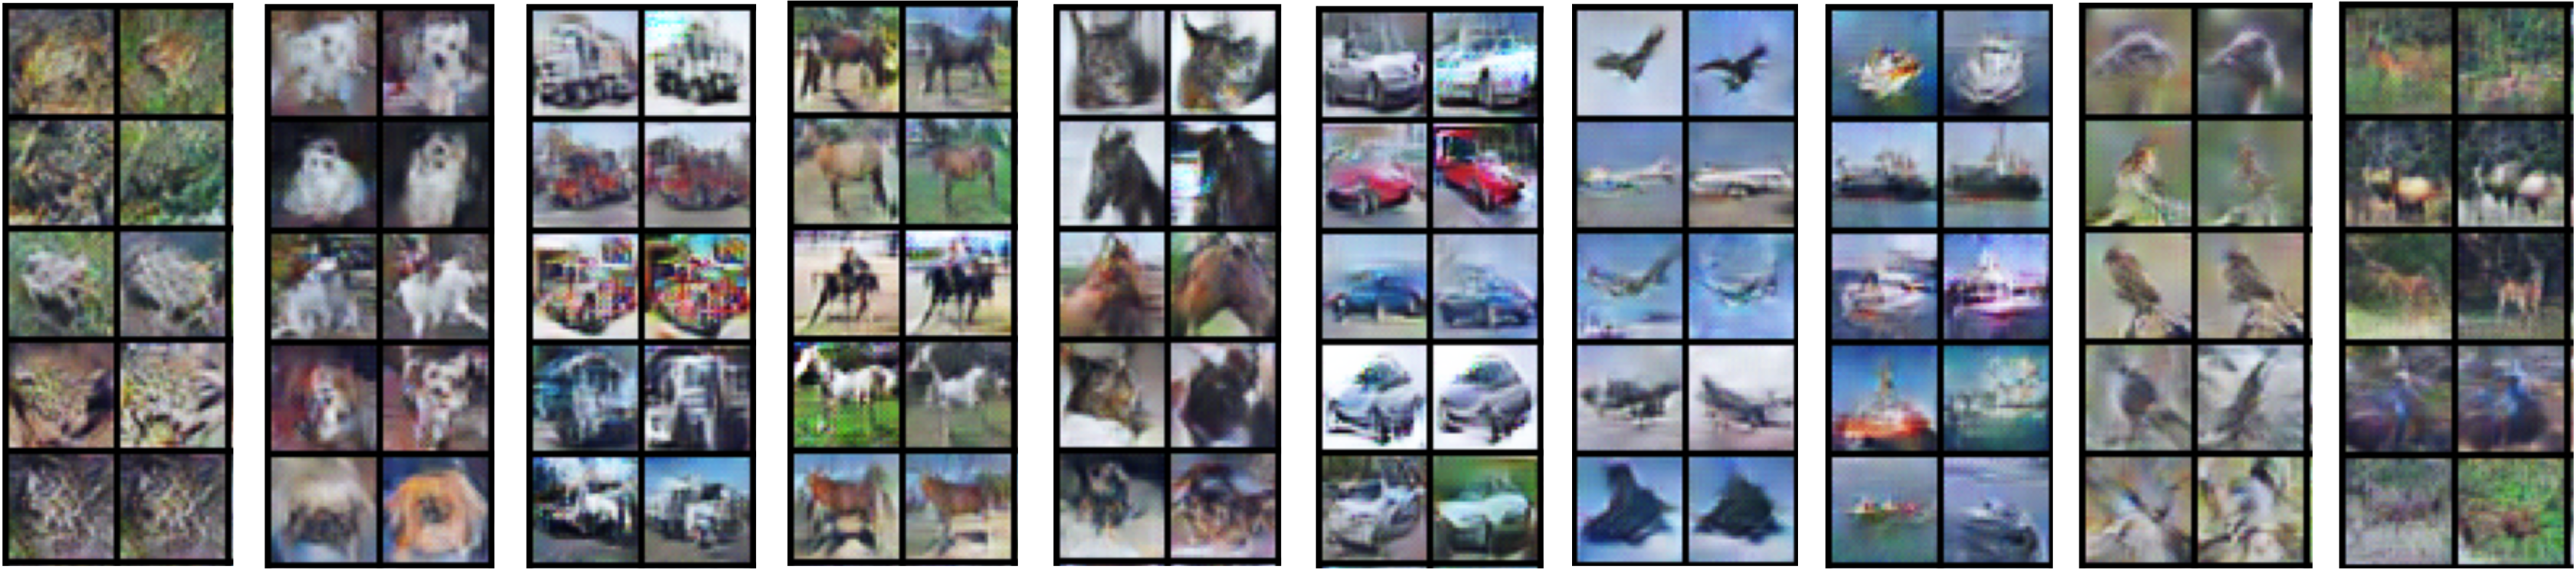
\includegraphics[width=0.95\textwidth]{\toplevelprefix/chapters/chapter5/figs/CIFAR10_generatedfromcluster.png}
    \caption{\small 使用u-CTRL从CIFAR-10的每个簇进行无监督条件图像生成。来自不同行的图像意味着从每个簇的不同主成分生成。}
    \label{fig:vis_clustering}
\end{figure}




% \section{其他变体} 
% 待定...

\section{总结与说明}
历史上,自编码一直是神经网络学习研究创新的重要驱动力之一,尽管深度学习最令人印象深刻的实际展示可能是在其他领域
(例如判别性分类,如AlexNet
\cite{krizhevsky2012imagenet},或使用GPT架构的生成建模
\cite{brown2020language})。
我们在本章中介绍的作品,特别是
\cite{Hinton504} 的工作,在神经网络在机器学习
研究领域不那么突出的时候,起到了研究兴趣的催化剂作用。
在现代实践中,自编码器仍然是许多用于生成高度结构化数据(如视觉数据、语音数据
和分子数据)的大规模系统的核心组件,特别是VQ-VAE方法
\cite{van-den-Oord2017-jr},它建立在我们
在 \Cref{sec:vae} 中讨论的变分自编码器
方法论之上。
自编码的核心问题由于其与表示学习的密切联系,
仍然具有至关重要的智力重要性,我们预计
随着训练和部署大型模型的效率变得越来越
重要,它将重新出现在实践研究人员的视野中。

本章后半部分介绍的材料基于一系列
关于闭环转录主题的最新工作:\cite{Dai-entropy-2022}、
\cite{pai2022pursuit}、\cite{tong2023incremental} 和 \cite{pmlr-v234-tong24a}。特别是,\Cref{sec:closed-loop-transcription} 基于 \cite{Dai-entropy-2022} 的开创性工作。此后,\cite{pai2022pursuit} 的工作为闭环框架提供了强有力的理论论证,至少在理想情况下是这样。\Cref{sec:class-wise-incremental} 和 \Cref{sec:sample-wise-incremental} 分别基于 \cite{tong2023incremental} 和 \cite{pmlr-v234-tong24a} 的工作。它们证明了闭环框架自然支持增量和持续学习,无论是在类别级还是样本级设置中。读者可以参考这些论文以获取更多的技术和实验细节。


\paragraph{浅层与深层神经网络,用于自编码及更多。}
在 \Cref{sub:nonlinear-pca} 中,我们讨论了Cybenko的通用近似
定理,以及它如何说明原则上,一个具有单个
隐藏层(和合适的逐元素非线性)的神经网络足以
逼近任何足够规则的目标函数。当然,在实践中,神经网络在实践中
占主导地位的主要架构原因是训练\textit{更深}神经网络
技术的改进。
为什么深度是必要的?
从根本的角度来看,深度分离的问题,即
构造一个更深的神经网络可以比浅层
网络以指数级更优的效率逼近给定类别的
目标函数的设置,
已经在理论文献中得到了广泛的研究:
例子包括 \cite{Telgarsky2016-sn,Bresler2020-xy,Venturi2021-qc}。
在实践中训练更深
网络的容易性从
理论的角度尚未得到同样令人满意的答案。
ResNets \cite{he2016deep} 代表了
使更深网络更容易训练的开创性实证工作,几乎在所有现代
架构中都以某种形式使用。理论研究主要集中在
非常深网络的训练能力上,通过初始神经正切核
\cite{Buchanan2021-sj,Martens2021-cx} 来量化,但这些研究并未对更深网络在训练中期
和后期的训练能力优势给出
重要见解(但请参见 \cite{Yang2021-gw} 作为试图解决此问题的一系列
研究的根源)。

\section{练习与扩展}

\begin{exercise}[流形展平的概念理解]
  考虑数据位于嵌入在 $\R^D$ 中的弯曲流形 $\cM$ 上(如
  3维空间中的曲面),如 \Cref{sub:nonlinear-pca} 的流形
  展平小节中所讨论的。
  在本练习中,我们将描述 \cite{Psenka-JMLR24} 中流形
  展平算法的基本要素。
  如果一个流形是欧几里得空间中的一个开集(或
  更一般地,是子空间中的一个开集),则称其为平坦的。

  \begin{enumerate}
    \item 假设流形 $\cM$ 是一个\textit{图}:这意味着 $\cM
      \subset \R^{D_1} \times \R^{D_2}$(比如说),并且存在一个函数 $F
      : \R^{D_1} \to \R^{D_2}$ 使得
      \begin{equation}
        \cM = \set{(\x, F(\x) \mid \x \in \R^{D_1})}.
      \end{equation}
      给出一个整数 $D_3$ 和一个映射 $f : \R^{D_1} \times \R^{D_2} \to \R^{D_3}$
      来展平 $\cM$,并描述从展平表示中相应的(无损)
      重构过程。
    \item 现在假设 $\cM$ 是一个一般的光滑流形。光滑流形
      具有在每个点附近都可以被子空间很好地近似的性质。用直观的术语描述如何通过将其与图相关联,在每个点局部地展平流形
      $\cM$。(\cite{Psenka-JMLR24} 的算法
      以一种允许它们被粘合在一起形成全局
      展平的方式,执行了这种局部展平过程的精炼版本。)
  \end{enumerate}
\end{exercise}


\begin{exercise}[复现闭环转录]

  在CIFAR-10数据集上实现一个用于表示学习的闭环转录流程,遵循
  \Cref{sec:closed-loop-transcription} 中的方法论。
  参考 \cite{Dai-entropy-2022} 获取有用的超参数和架构
  设置。复现 \Cref{fig:justifyz=z} 中的结果。


\end{exercise}

\end{document}